\documentclass[journal]{IEEEtran}
\usepackage[colorlinks,linkcolor=blue,anchorcolor=blue,citecolor=blue]{hyperref}
\usepackage{algorithm}
%\usepackage[linesnumbered,boxed]{algorithm2e}
\usepackage[algo2e,vlined,linesnumbered]{algorithm2e}
\usepackage{amsmath}
\usepackage{amssymb}
\usepackage{balance}
\usepackage{booktabs}
\usepackage{epsfig}
\usepackage{graphicx}
\usepackage{graphics}
\usepackage{mathptm}
\usepackage{subfigure}
\usepackage{times}

%\pdfpagewidth=8.5in
%\pdfpageheight=11in
%\setlength{\textheight}{9.45in}
%\setlength{\floatsep}{0pt}% Remove \textfloatsep
%\setlength{\textfloatsep}{0pt}% Remove \textfloatsep
%\setlength{\intextsep}{0pt}% Remove \textfloatsep
%\setlength{\dbltextfloatsep}{0pt}% Remove \textfloatsep
%\setlength{\dblfloatsep}{0pt}% Remove \textfloatsep
%\setlength{\abovecaptionskip}{0pt}% Remove \textfloatsep
%\setlength{\belowcaptionskip}{0pt}% Remove \textfloatsep
%\def\wrapper#1{}
%%%%%%%%%%%%%%%%%%%%%%%%%%%%%%%%%%%%%%%%%%%%%%%%%%%%%%%%%%%%%%%%%%%%%
% ATTENTION: Our fax number for sending the proofs is: (858) 822-5003
%%%%%%%%%%%%%%%%%%%%%%%%%%%%%%%%%%%%%%%%%%%%%%%%%%%%%%%%%%%%%%%%%%%%%

\newtheorem {theorem}{Theorem}
\newtheorem {definition}{Definition}
\newtheorem {lemma}{Lemma}
\newtheorem {proposition}{Proposition}
\newtheorem {fact}{Fact}
%\renewcommand{\algorithmicrequire}{\textbf{Input:}}
%\renewcommand{\algorithmicensure}{\textbf{Output:}}
\hyphenation{conta-mination}

%\newcounter{reviewercount}
%\newcounter{commentcount}
%\newcommand{\reviewer}{\bigskip\noindent {\bf COMMENTS OF REVIEWER
%    \#\refstepcounter{reviewercount}\thereviewercount.}
%    \setcounter{commentcount}{0}\par\rm\em
%}

%\newcommand{\aeditor}%
%   {\bigskip\noindent {\bf COMMENTS OF THE ASSOCIATE EDITOR}%
%   \setcounter{commentcount}{0} }
%
%\newcommand{\rcomment}{\bigskip\par\noindent{\bf Comment
%   \refstepcounter{commentcount}
%   \thereviewercount.\thecommentcount: }\rm\em
%}

%\newcommand{\response}{\smallskip\par\noindent{\bf Response: }\em\rm }

%\def\wrapper#1{}


\begin{document}
% paper title

%\setlength{\leftmargini}{1.5em} \setlength{\leftmarginii}{1.5em}
%\setlength{\leftmarginiii}{1.5em}

\title{AARF: Any-Angle Routing for Flow-Based Microfluidic Biochips\thanks{The work of H. Yao was supported in part by the National Natural Science Foundation of China (61674093) and Tsinghua University Initiative Scientific Research Program (20141081203).
The work of T.-Y. Ho was supported in part by the Ministry of Science and Technology of Taiwan, under Grant MOST 105-2221-E-007-118-MY3 and 104-2220-E-007-021 and in part by the Technical University of Munich-Institute for Advanced Study, funded by the German Excellence Initiative and the European Union Seventh Framework Program under grant agreement no 291763.
The work of Y. Cai was supported by the National Natural Science Foundation of China (61274031).}
}

\author{
\qquad Kailin Yang\thanks{Kailin Yang, Hailong Yao, and Yici Cai are with the Department of Computer Science and Technology, Tsinghua University, Beijing 100084, China. E-mails: hailongyao@tsinghua.edu.cn, ykl14@mails.tsinghua.edu.cn, caiyc@tsinghua.edu.cn.}
\qquad Hailong Yao
\qquad Tsung-Yi Ho\thanks{Tsung-Yi Ho is with Department of Computer Science, National Tsing Hua University. E-mail: tyho@cs.nthu.edu.tw.}
\qquad Kunze Xin\thanks{This work was done during Mr. Kunze Xin's internship at Tsinghua University. E-mail: xkz218@sina.com.}
\qquad Yici Cai
\thanks{Copyright $\copyright$ 2016 IEEE. Personal use of this material is permitted.
However, permission to use this material for any other purposes must be obtained from the IEEE by sending an
email to pubs-permissions@ieee.org.}
}

\markboth{IEEE TRANSACTIONS ON COMPUTER-AIDED DESIGN OF INTEGRATED CIRCUITS AND SYSTEMS, VOL. XX, NO. Y, MONTH XX, 2016.}.

\maketitle
%\vspace{-30.0cm}
\begin{abstract}
Flow-based microfluidic biochips are promising with significant applications for automating and miniaturizing laboratory procedures in biochemistry. Automated design methods for flow-based microfluidic biochips are becoming increasingly important due to the advancement in both integration scale and design complexity for complicated biochemical applications. Though the multilayer soft lithography fabrication provides flexibility to route both flow and control channels in any angle, existing routing algorithms still adopt Manhattan routing metrics, which design channel in either vertical or horizontal direction only. Moreover, based on the computational fluid dynamics (CFD) analysis, rectilinear channels with 90$^\circ$ bends have the following issues: (1) reduced the fluidic flow rate, which degrades the performance of the biochip and may even result in the erroneous outcome of the whole procedure, and (2) increased pressure at the right-angle bend, which negatively affects the reliability of the biochip. To fully utilize the routing flexibility, this paper proposes the first any-angle routing algorithm for flow-based microfluidic biochip, called AARF. Computational simulation results show that compared with traditional Manhattan routing method, the proposed AARF significantly improves the total wirelength and total effective wirelength (considering the turning angles) by 19.28\% and 53.04\%, respectively, which prove the effectiveness of the AARF routing flow.

\end{abstract}

\begin{keywords}
Flow-based microfluidic biochips, Any-angle routing, Dynamic programming, Computational fluidic dynamics (CFD) simulation
\end{keywords}

%\vspace{-0.1cm}
\section{Introduction}
\label{sec:intro}
%\vspace{-0.1cm}

\begin{figure}[t]
%%\vspace{-0.45cm}
\centering
\subfigure[]
{
%\label{fig:RC:a}
\begin{minipage}[b]{0.8\columnwidth}
\centering
\resizebox{\columnwidth}{!}{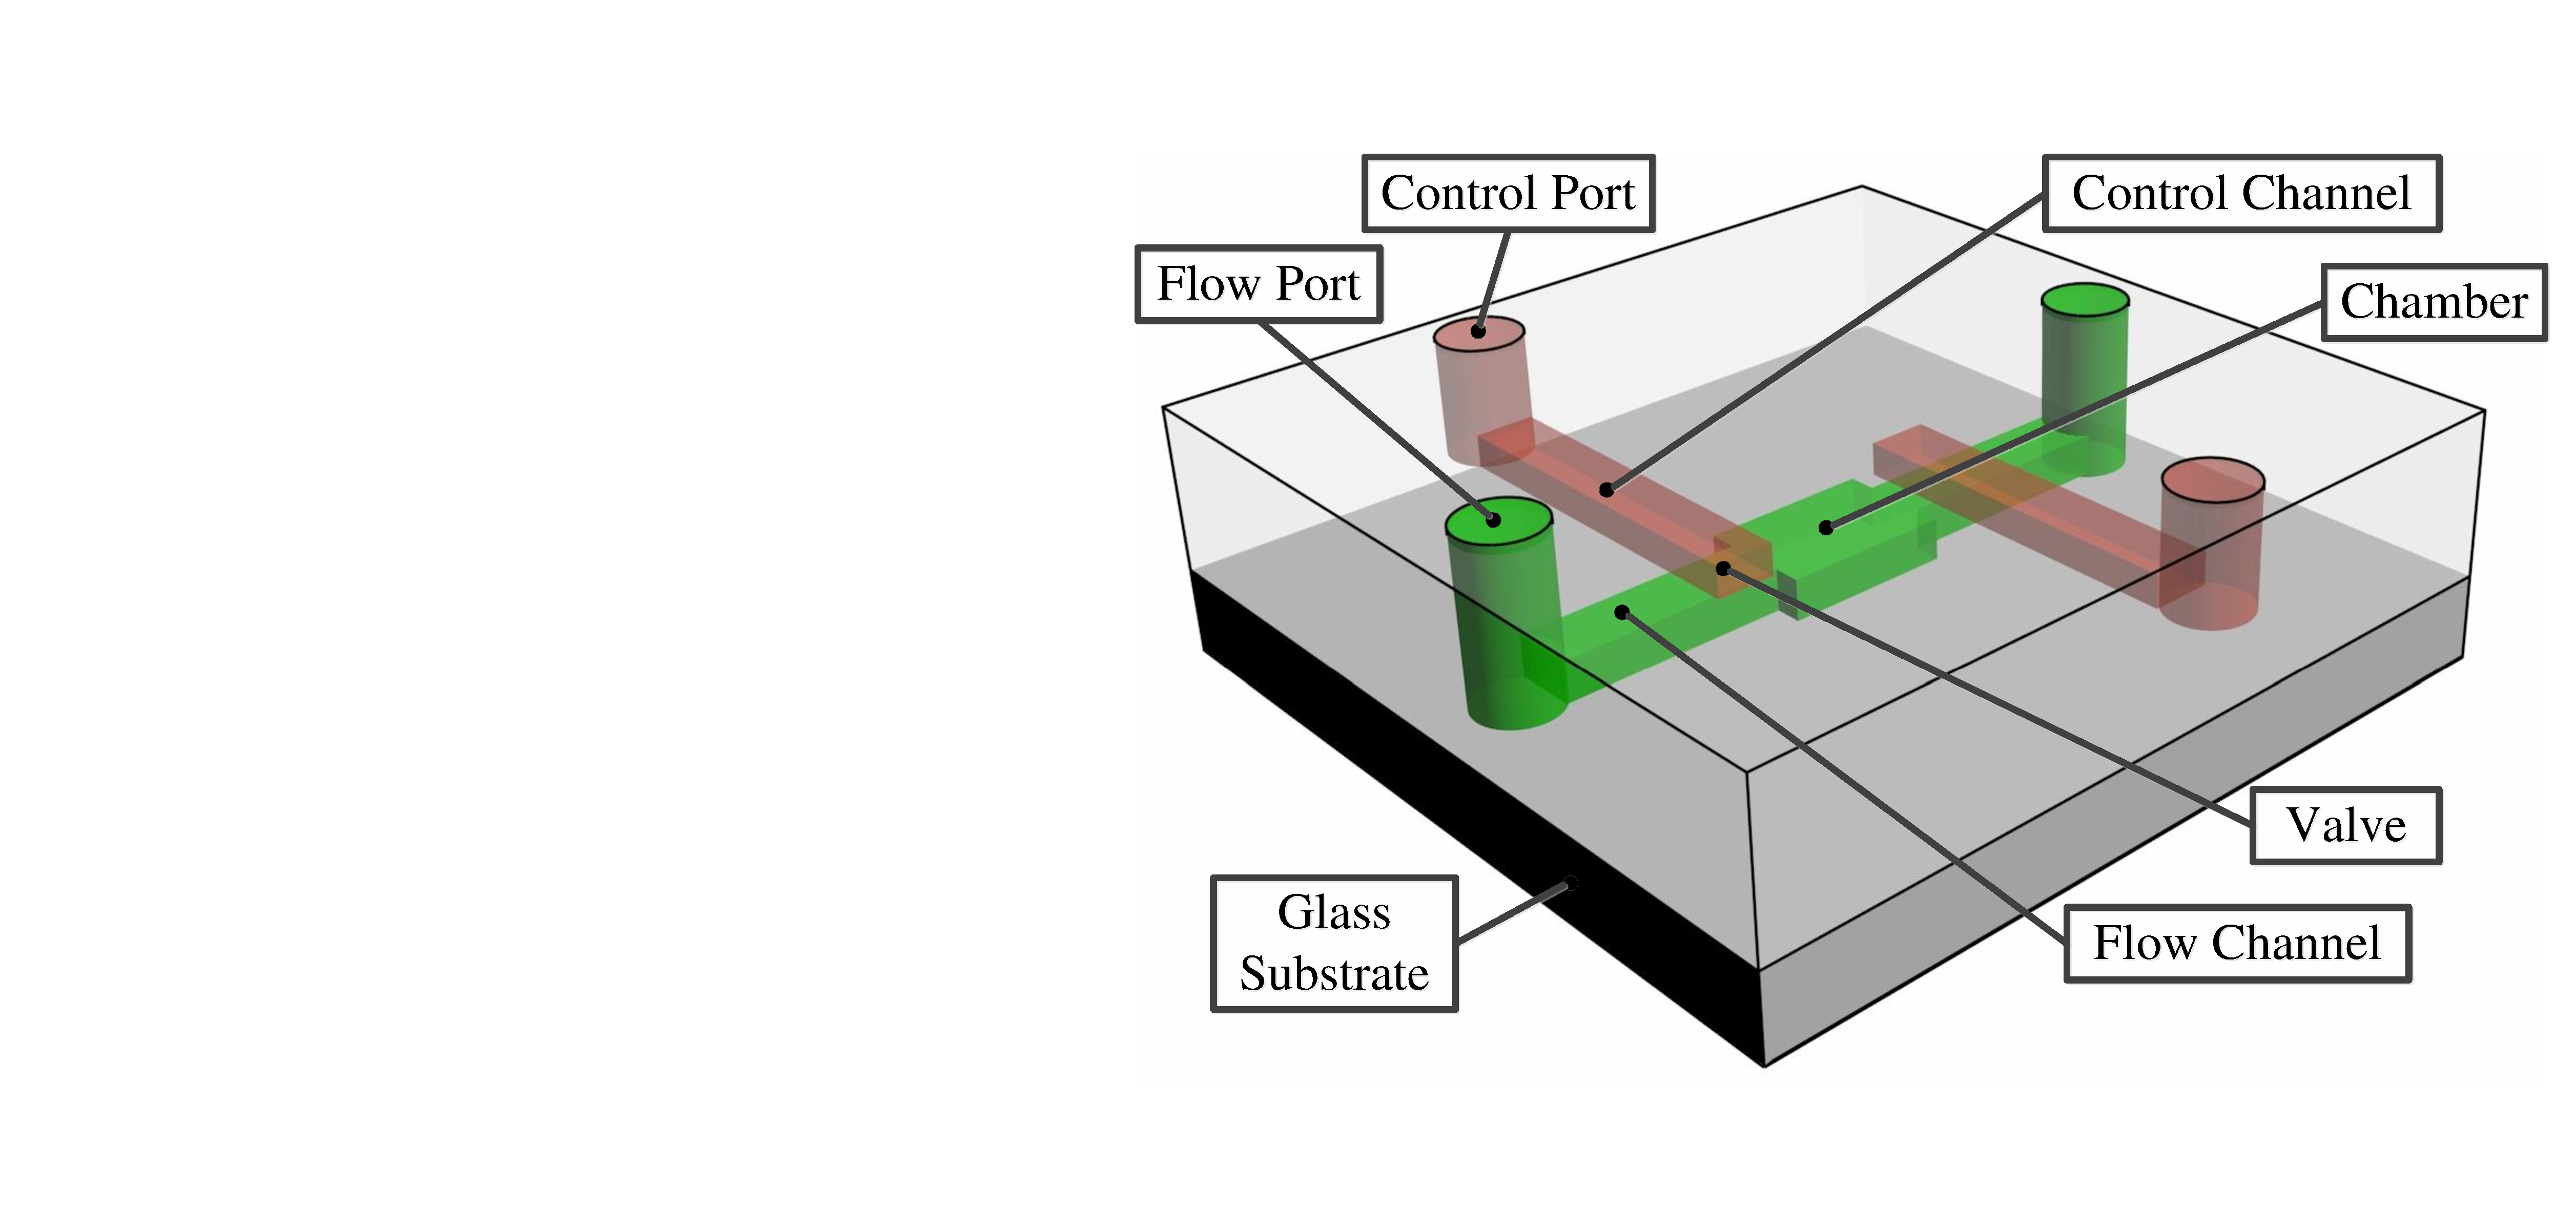
\includegraphics[width=0.8\columnwidth, angle=0]{./Figs/biochip.pdf}}
\end{minipage}%
}%
\hfil
%%\vspace{-0.25cm}
\subfigure[]
{
%\label{fig:RC:b}
\begin{minipage}[b]{0.7\columnwidth}
\centering
\resizebox{\columnwidth}{!}{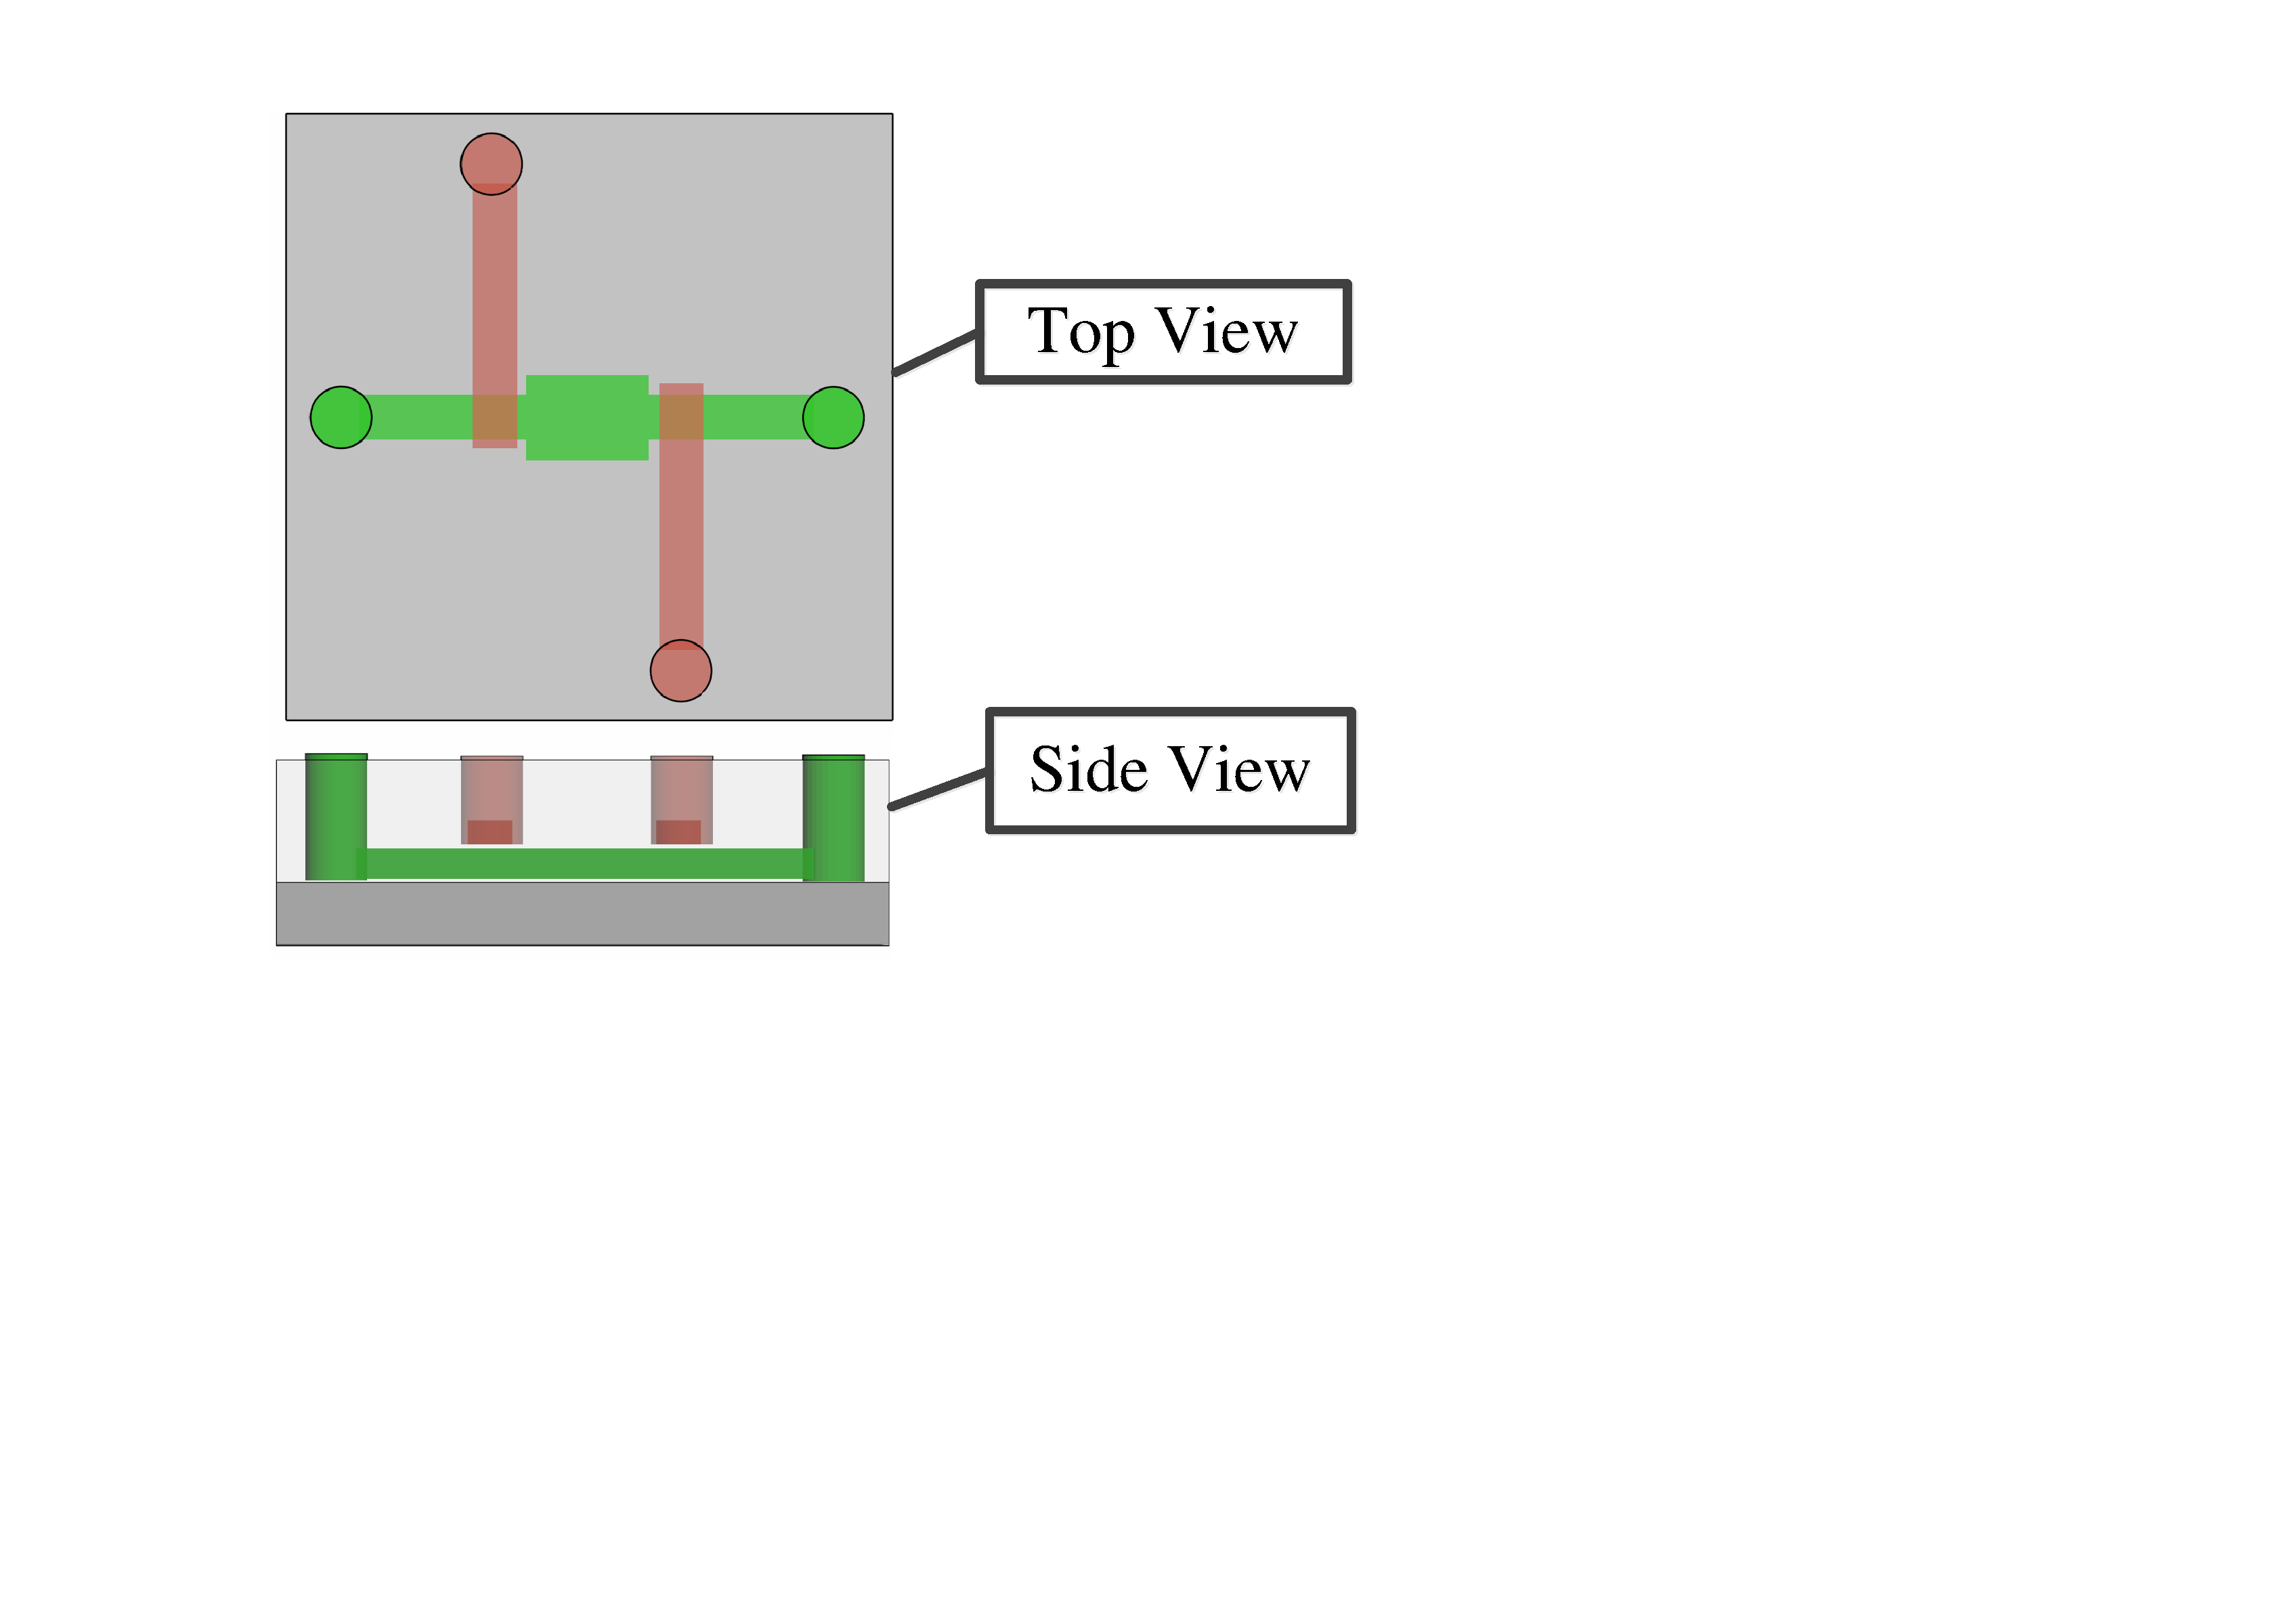
\includegraphics[width=0.7\columnwidth, angle=0]{./Figs/TopSideView.pdf}}
\end{minipage}%
}%
%%\vspace{-0.2cm}
\caption{Schematic of flow-based biochip with different perspective views. (a) 3D view, and (b) Top and side views. }
\label{fig:schematic}
\vspace{-0.35cm}
\end{figure}


Microfluidic biochip, also known as Lab-on-a-Chip (LoC), has emerged as 
a revolutionary technique toward miniaturization and automation of the laboratory
procedures in biochemistry \cite{Balagadde:2005bk,Whitesides:2006jj,Yager:2006kd}. 
LoC integrates different biochemical analysis modules, such as mixer, separator, chamber, etc., 
into a single chip, and hence reduces samples/reagents to microliter or even nanoliter scale \cite{Thorsen:2002ec,Mark:2010fk}.
Noticeable merits of microfluidic biochips over traditional laboratory platforms include: (1) greatly saving the assay cost by reducing expensive samples/reagents to nano-liter or pico-liter volume, (2) effectively integrating the automatic control logic for reduced human intervention and labor cost, (3) significantly increasing sensitivity, accuracy and throughput, (4) essentially facilitating portability for point-of-care diagnostics, and (5) naturally enabling microscale assays (e.g., single-cell culture, capture and analysis) that are infeasible by traditional macroscale approaches.
According to Research and Markets, the global biochips market is expected to grow at a compound annual
growth rate (CAGR) of 22.8\% from 2013 to 2019, and will reach \$52 Billion by 2019 \cite{RandM}.
Applications of biochips cover many different fields, such as diagnostics and treatment, drug discovery and development, biological research, forensic analysis, agriculture, environmental sensors, food inspection, etc. For example, microfluidic biochips are recently designed for point-of-care HIV/AIDS and cancer diagnosis \cite{Watkins:2013id,rice}.


\begin{figure}[htbp]
%%\vspace{-0.45cm}
\centering
\subfigure[]
{
%\label{fig:RC:a}
\begin{minipage}[b]{0.9\columnwidth}
\centering
\resizebox{\columnwidth}{!}{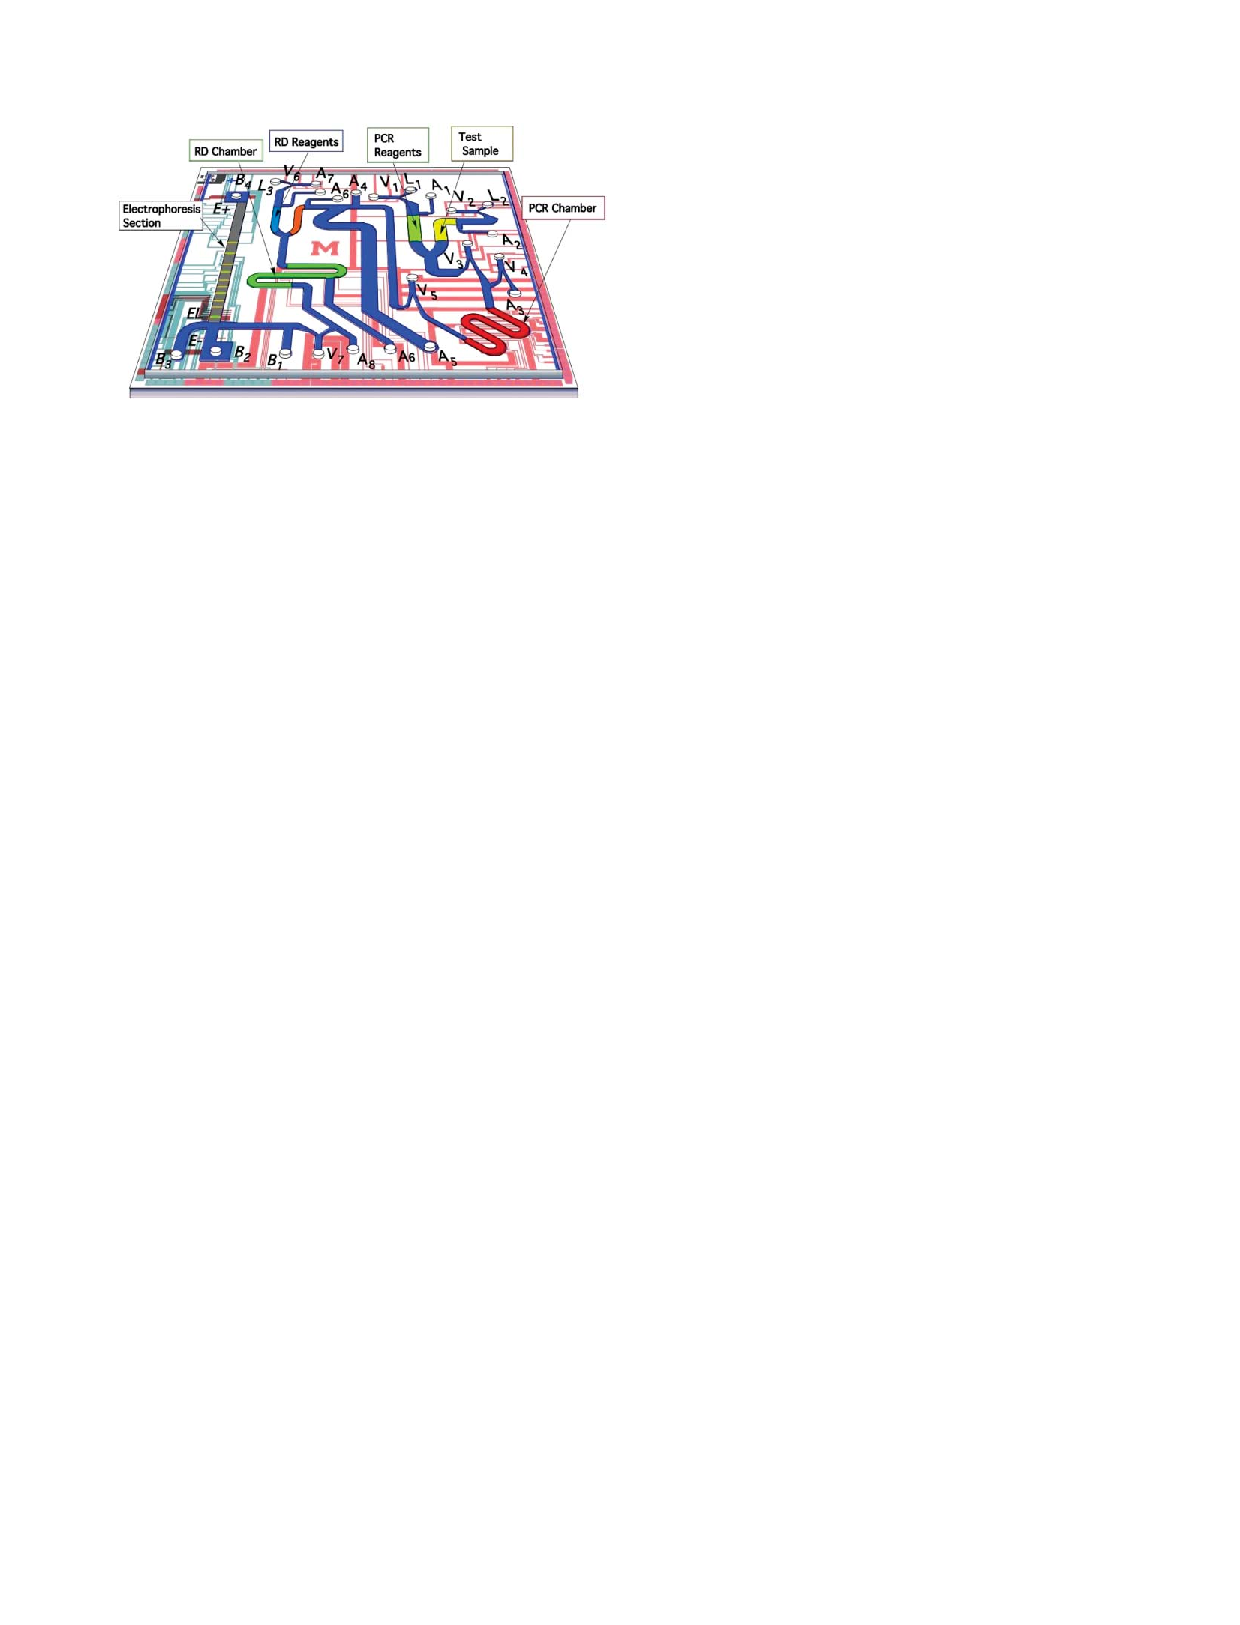
\includegraphics[width=0.9\columnwidth, angle=0]{./Figs/anyangleExampleA.pdf}}
\label{fig:aaexample:a}
\end{minipage}%
}%
\hfil
%%\vspace{-0.25cm}
\subfigure[]
{
%\label{fig:RC:b}
\begin{minipage}[b]{0.9\columnwidth}
\centering
\resizebox{\columnwidth}{!}{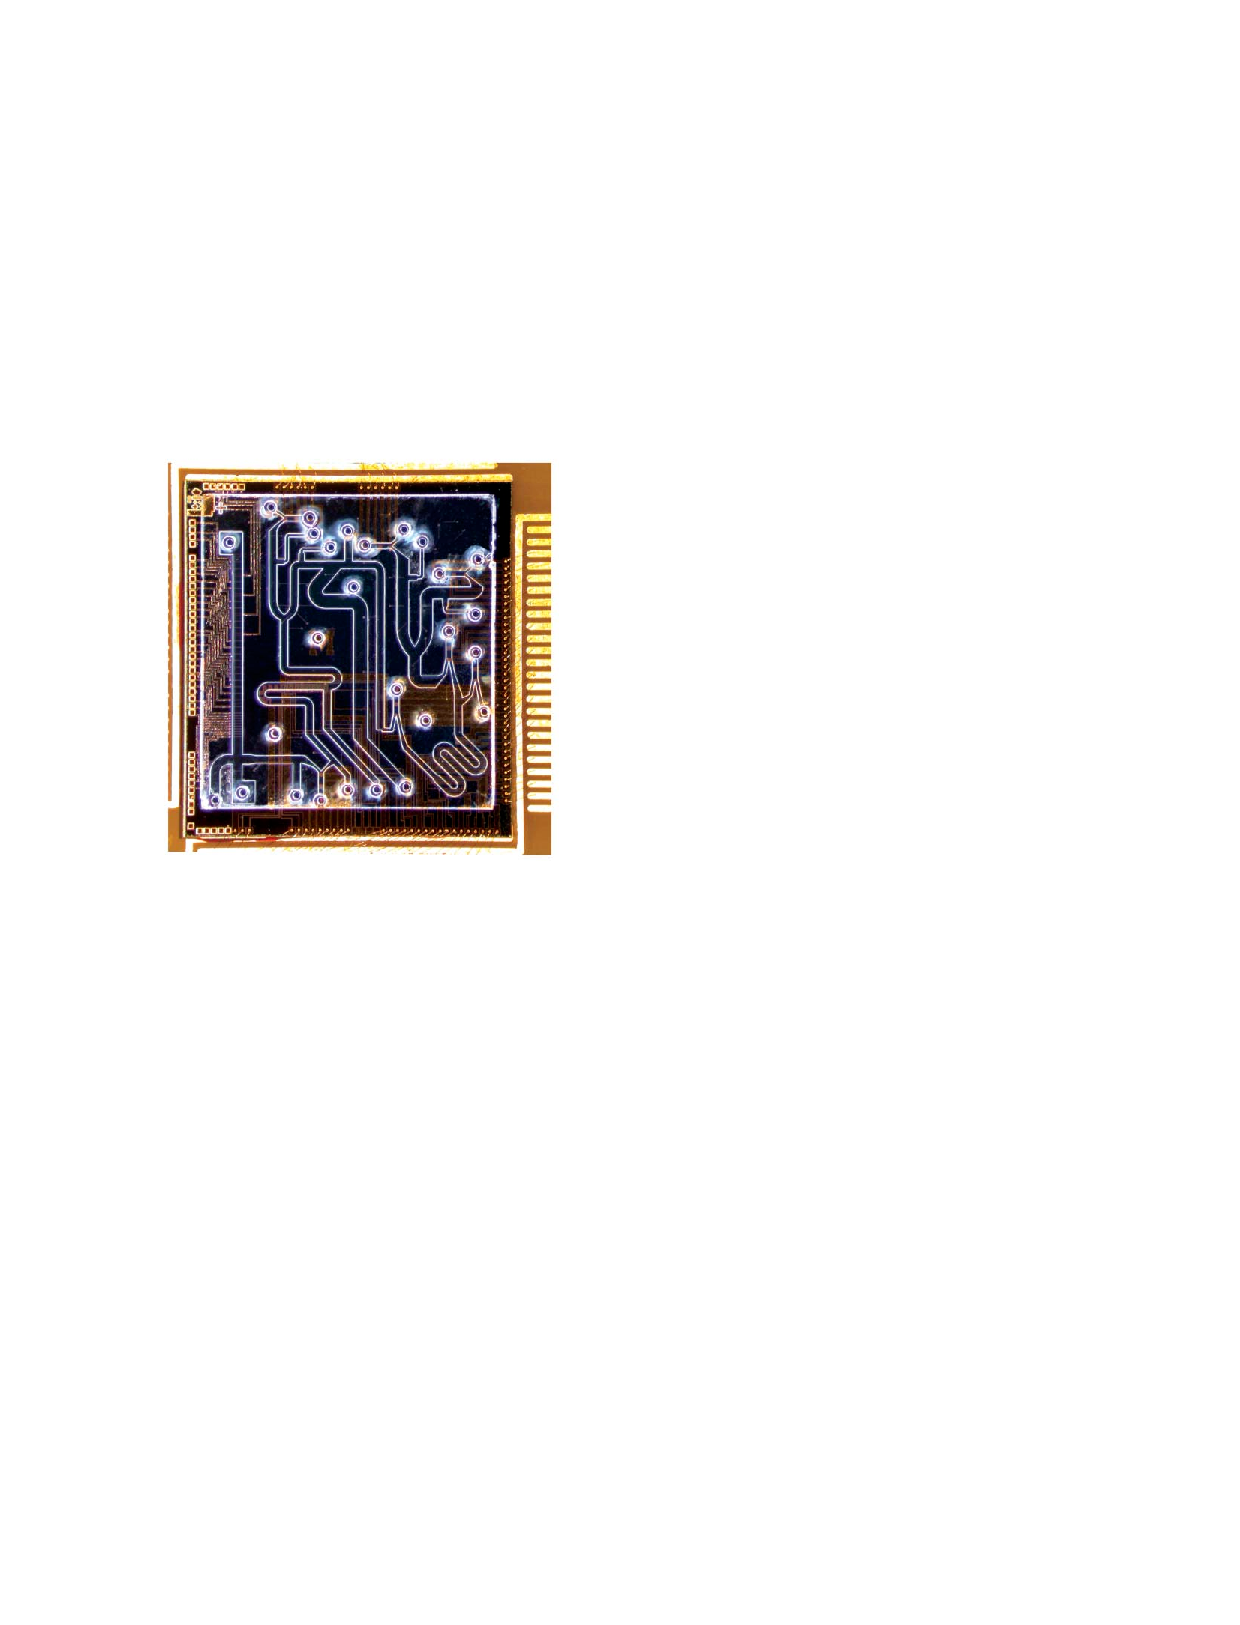
\includegraphics[width=0.9\columnwidth, angle=0]{./Figs/anyangleExampleB.pdf}}
\label{fig:aaexample:b}
\end{minipage}%
}%
%\vspace{-0.2cm}
\caption{Microfluidic chip example with any-angle flow channels. (a) Schematic representation, and (b) Photograph of the assembled device. }
\label{fig:aaexample}
%\vspace{-0.25cm}
\end{figure}

Flow-based microfluidic biochip is one of the most commonly used microfluidic biochips, which is fabricated using {\em multilayer soft lithography} (MSL) technology. 
In flow-based microfluidic biochips, microfluidic functional units are fabricated by elastomer material (polydimethylsiloxane, PDMS) \cite{Thorsen:2002ec,Rogers:2005vu}. 
Figure~\ref{fig:schematic} shows the schematic of flow-based microfluidic biochip, which consists of two functional layers \cite{QinRu:2016}. 
In the figure, the 3D view of a demonstrative chamber for cell culture is shown in Figure~\ref{fig:schematic}(a), and the corresponding top and side views are shown in Figure~\ref{fig:schematic}(b). 
On top of the glass substrate, there are two PDMS layers: (1) {\em flow layer} for fluidic sample/reagent transportation, and (2) {\em control layer} for enforcing the controlling logic through control channels. Both control and flow channels are connected to input/output ports, which are punched holes through the PDMS material.
A {\em microvalve} ({\em valve} for short) is formed between control and flow channels at their intersection area.
To switch the valve, external pressure is injected through {\em control port} (also called {\em control pin}). 
Then hydraulic or pneumatic pressure ($\sim$10 psi) will be conducted through control channel to the valve, squeezing the elastomer down to seal the flow channel. 
When external pressure is released, the elastomer will restore back, 
and the fluidic flow will resume due to external pressure from the {\em flow port}.

Different complex units can be formed in the biochip by combining several valves, such as micropumps, 
mixers, multiplexers, etc \cite{Mark:2010fk}. By controlling these units 
through different actuation patterns on valves, fluids (i.e., samples/reagents) are 
manipulated to transport in flow channels for different operations, 
e.g., splitting, mixing, filtering, metering, etc. Thus, an assay can be realized by executing 
the sequential fluidic operations automatically in a programmed way \cite{Squires:2005vb}.
With the advancements of fabrication techniques in multilayer soft 
lithography, the size of valves has been reduced to 
$6 \times 6\mu m^2$ \cite{Unger:2000gm,Araci:2012gl}. And the valve density 
has reached 1 million valves per $cm^2$, which makes manual design impossible
for the microfluidic very large-scale integration (mVLSI). 
Due to the ever increasing complexity in both bioassays and integration scale, 
computer-aided design (CAD) methods are becoming necessary 
for reliable biochip designs to achieve correct functionality and 
reduced turnaround time.

Though PDMS is a flexible material for molding, pressure propagation through the control channel is very slow from the control pin to the corresponding valve(s) \cite{Lim:2010iq}. 
Moreover, the propagation time will significantly increase due to reduced driving 
force especially in portable microfluidic devices. This critical issue also existed in flow channels.
Therefore, flow-based microfluidic biochips typically adopt any-angle flow channels for better performance in the assay experiments. Figure~\ref{fig:aaexample}(a)(b) shows an example of an integrated microfluidic device with any-angle flow channels for influenza and genetic analyses in both schematic and photographic view \cite{Pal:2005}. However, existing automated design methods for flow-based microfluidic biochips are still based on Manhattan metrics, which compute Manhattan channels on both flow and control layers. 
In this paper, we propose the first any-angle routing method, called {\bf AARF}, which obtains shorter channel lengths compared with Manhattan routing. Moreover, the fluidic flow rate is further enhanced by 
the proposed dynamic programming approach. From the computational fluidic dynamics (CFD) analysis, the computed any-angle channel has much better performance compared with the corresponding Manhattan channel.

\begin{figure}[htbp]
	%%\vspace{-0.45cm}
	\centering
	\subfigure[]
	{
		%\label{fig:RC:a}
		\label{fig:result:a}
		\begin{minipage}[b]{0.48\columnwidth}
			\centering
			\resizebox{\columnwidth}{!}{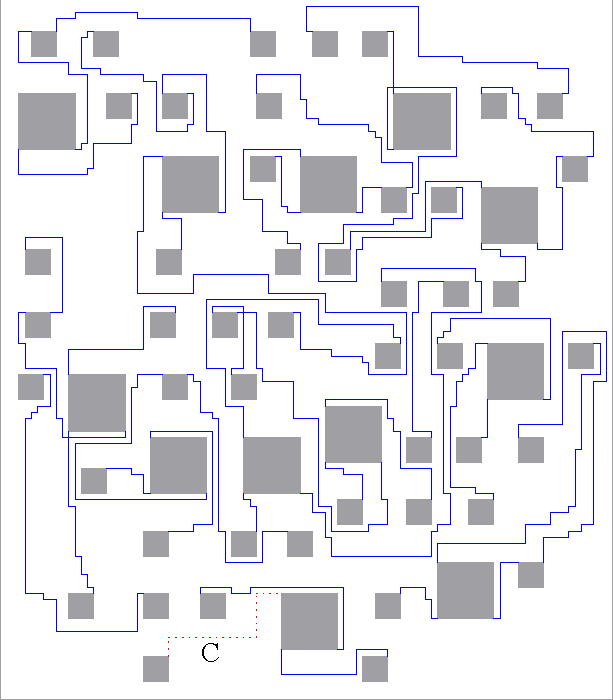
\includegraphics[width=0.48\columnwidth, angle=0]{./Figs/MR.pdf}}
		\end{minipage}%
		
	}%
	\hfil
	%%\vspace{-0.25cm}
	\subfigure[]
	{
		%\label{fig:RC:b}
		\label{fig:result:b}
		\begin{minipage}[b]{0.48\columnwidth}
			\centering
			\resizebox{\columnwidth}{!}{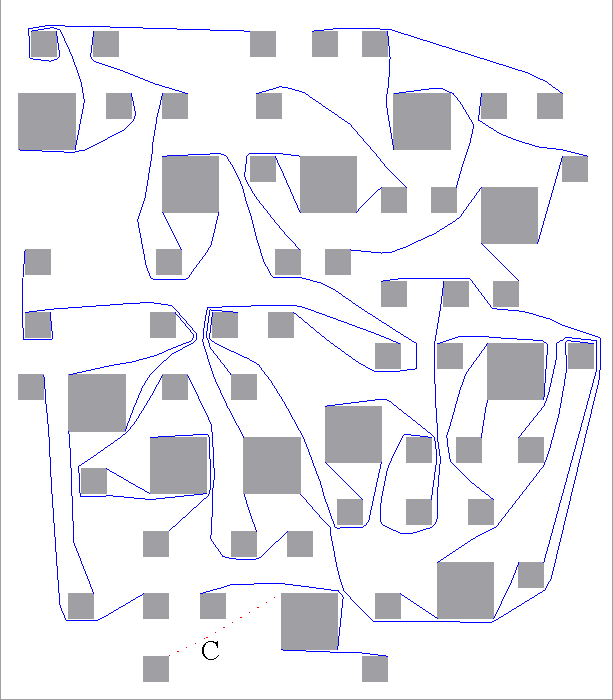
\includegraphics[width=0.48\columnwidth, angle=0]{./Figs/AARF.pdf}}
		\end{minipage}%
	}%
	%%\vspace{-0.2cm}
	\caption{Routing result of (a) Manhattan routing, and (b) AARF. }
	\label{fig:result}
	%%\vspace{-0.25cm}
\end{figure}

Figure~\ref{fig:result:a} shows the rectilinear channels designed using the traditional Manhattan routing method, and Figure~\ref{fig:result:b} shows the any-angle routing result from our AARF router. 
From CFD simulation reports by ANSYS Fluent software \cite{fluent}, the velocity magnitude (i.e., flow rate) of channel C by Manhattan routing is 0.0053 m/s (see Figure~\ref{fig:result:a}), whereas that of any-angle routing from AARF is 0.0316 m/s. That is, around 6$\times$ improvements in flow rate can be obtained using the proposed any-angle routing method.
To the best of our knowledge, this paper is the first work on any-angle routing considering the flow rate for flow-based microfluidic biochips. 
In the past decade, noticeable advances have been made in CAD methodology 
for digital microfluidic biochips, including
resource binding, operation scheduling, module placement, and droplet routing \cite{SU:2004ul,Cho:2008dk,SU:2005db,Yuh:2007kd,Huang:2011iy}. However, only a few works addressed the CAD problems for flow-based biochips. Minhass et al. presented 
a constraint programming based synthesis method for flow-based biochips \cite{Minhass:2012th}. Lin et al. presented a flow channel routing 
method, which simultaneously minimizes the total length and the maximum
length of flow channel \cite{Lin:2014ex}. Amin et al. presented the first control-layer 
routing method for flow-based microfluidic biochips \cite{Amin:2009eh}. 
Minhass et al. presented a control synthesis method, which addresses 
the assignment from valves to control pins for minimized number of control pins 
 \cite{Minhass:2013cm}.
In \cite{Hu:2014dt}, a control-layer routing algorithm is presented to minimize the 
pressure-propagation delay of the control signals. 
In \cite{Yao:2015}, the length-matching routing constraints are enforced during the routing for control-layer channels. 
In \cite{wq:2016}, placement and routing methods for flow-based microfluidic biochips
are proposed based on the classic sequence-pair-based representation. 
However, no existing works consider any-angle routing for flow-based microfluidic biochip to significantly enhance flow rate. 

In this paper, we propose the first any-angle routing method for flow-based microfluidic 
biochips, called {\bf AARF}, which designs the non-rectilinear flow channels for 
enhanced fluidic flow rate. With the constrained Delaunay triangulation structure, we proposed the dynamic-programming-based approach to further enhance the flow rate in non-rectilinear channels based on CFD metrics. 
Moreover, the total channel lengths are also significantly reduced compared with 
the Manhattan routing results. Major contributions of the paper are listed as follows.

\begin{itemize}
%\vspace{-0.2cm}
\item The first any-angle routing method is proposed with enhanced fluidic flow rate and 
minimized total effective channel length, i.e., weighted wirelength considering the turning angles of non-rectilinear channels.
%\vspace{-0.2cm}
\item Constrained Delaunay triangulation structure is computed for the coarse path searching procedure, and iteratively updated with newly routed flow channels.

\item Dynamic-programming-based routing approach is proposed to optimize the total effective wirelength, which significantly improves the flow rate.
%\vspace{-0.2cm}
\item A theoretical model is adopted in any-angle routing process to efficiently compute the effective wirelength from the turning angles in the non-rectilinear flow channels. 
%\vspace{-0.2cm}
\item CFD simulations are performed to accurately evaluate the flow rates 
of the non-rectilinear channels obtained by AARF vs. the rectilinear channels from the 
existing Manhattan routing method.
%\vspace{-0.2cm}
\end{itemize}

The remainder of this paper is organized as follows. 
Section~\ref{sec:formulation} presents the problem formulation. 
Section~\ref{sec:overview} presents the overall flow of the proposed any-angle routing method AARF. 
Section~\ref{sec:dtg} presents the details of constrained Delaunay triangulation graph.
Section~\ref{sec:toporoute} presents the coarse path searching process on the related search graph.
Section~\ref{sec:dp} presents the dynamic-programming-based routing method for minimized total effective wirelength.
Section~\ref{sec:prca} presents the pseudocode of AARF and the analysis of its runtime complexity.
Section~\ref{sec:exp} presents and discusses the computational simulation results. 
Finally, conclusion is drawn in Section~\ref{sec:cln}.

%\vspace{-0.1cm}
\section{Preliminaries and Problem Formulation}
\label{sec:formulation}

\subsection{Effective Channel Length}
\label{subsec:pre}

\begin{figure}
%\vspace{-0.1cm}
\label{fig:overview}
\centering
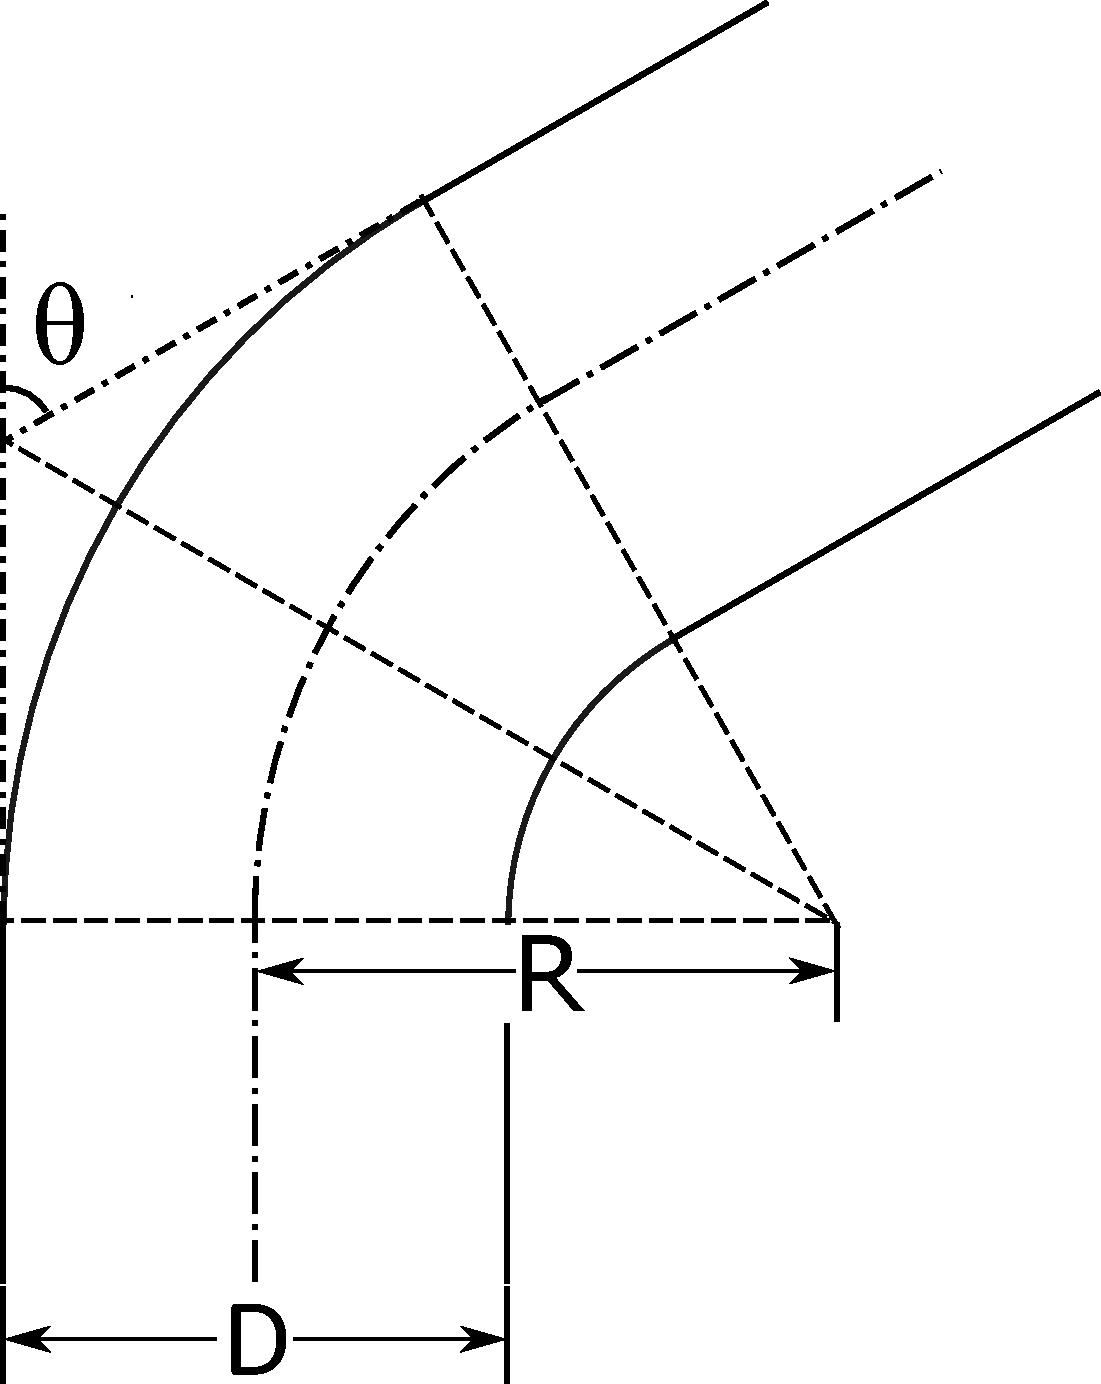
\includegraphics[width=0.6\columnwidth, angle=0]{./Figs/turnangleDef.pdf}
\vspace{-0.2cm}
\caption{Definition of a turning angle formed by two channel segments along with an arc channel.}
\label{fig:turnangle}
%\vspace{-0.55cm}
\end{figure}

According to simulation results of computational fluid dynamics (CFD), the flow rate is 
mainly affected by layout pattern of the channel, especially the turns along the channel. 
Here we define {\em turning angle} as supplement of the angle formed by two segments at
the turn.
Figure~\ref{fig:turnangle} shows an example, where angle $\alpha$ is the turning angle of 
the elbow.
Generally, the more turns a channel contains, the slower the flow rate would be; 
and the larger the turning angle is, the slower the flow rate would be.
Besides the influence on the flow rate, a large turning angle also increases 
the pressure against the channel at the elbow, which is similar to the river 
channel erosion at the river bend. Such increased pressure against the channel's 
sidewall is hazardous to the lifetime of the PDMS channel in flow-based microfluidic 
biochips. Therefore, in this paper we propose the first any-angle routing method, AARF, to 
avoid elbows with large turning angles in the computed flow channels.

In AARF, we adopt a classical method in the CFD field to convert the turning angles 
into effective channel lengths such that the impact of turning angles could be efficiently evaluated. 
The effective channel length L' of a turning angle is defined as follows:

\begin{equation}
\label{eqn:effl}
L' = \frac{\xi}{\lambda} \cdot D
%\vspace{-0.15cm}
\end{equation}

\noindent where $D$ denotes the width of the channel. $\lambda$ is the 
{\em coefficient of frictional resistance}, which is determined by the Reynolds number, the status of the fluid, and the roughness of the channel. 
And $\xi$ is the {\em coefficient of local resistance}, which is affected by the turning angle $\theta$ and is computed as follows:

\begin{equation}
\xi = [\alpha+\beta \cdot (\frac{D}{R})^{\tau}] \cdot \frac{\theta}{90}
%\vspace{-0.15cm}
\end{equation}

\noindent where $\theta$ is the turning angle, $D$ is the width of the channel, $R$ is the radius of curvature of the turn (see Figure~\ref{fig:turnangle}). $\alpha$, $\beta$, and $\gamma$ are experimentally determined parameters.
% which are set to be 0.131, 0.159 and 3.5, respectively.
%{\bf KY: the real value of parameters are hided.}
When the effective channel lengths are computed for the turns along a channel, 
the {\em total effective wirelength} represents sum of the actual channel lengths 
and the effective channel lengths of the turns. 
During the routing process, the total effective wirelength is used to measure the 
solution quality of the computed channels with elbows. In this way, the proposed routing 
method can design the channels with relatively shorter length and elbows of smaller turning angles. 

\subsection{Problem Formulation}
\label{subsec:for}

Considering the effective channel length for enhanced fluidic flow rate, the any-angle routing problem for flow-based microfluidic biochips can be formulated as follows:

\textbf{Input:}
A list of nets (pairs of routing terminals) to be connected, a set of functional modules with routing terminals, a set of rectilinear routing blockages, a set of design rules for routing channels, and the biochip's design boundary.

\textbf{Objective:}
Find the channel routing solution for all the nets with minimized total effective wirelength computed by Equation~(\ref{eqn:effl}).

\textbf{Constraint:}
(1) The computed flow channel can be in any angle rather than just Manhattan. (2) The minimum channel width and the minimum channel spacing constraints must be satisfied.

%\vspace{-0.1cm}
\section{Algorithm Overview}
\label{sec:overview}

\begin{figure}
%\vspace{-0.1cm}
\label{fig:overview}
\centering
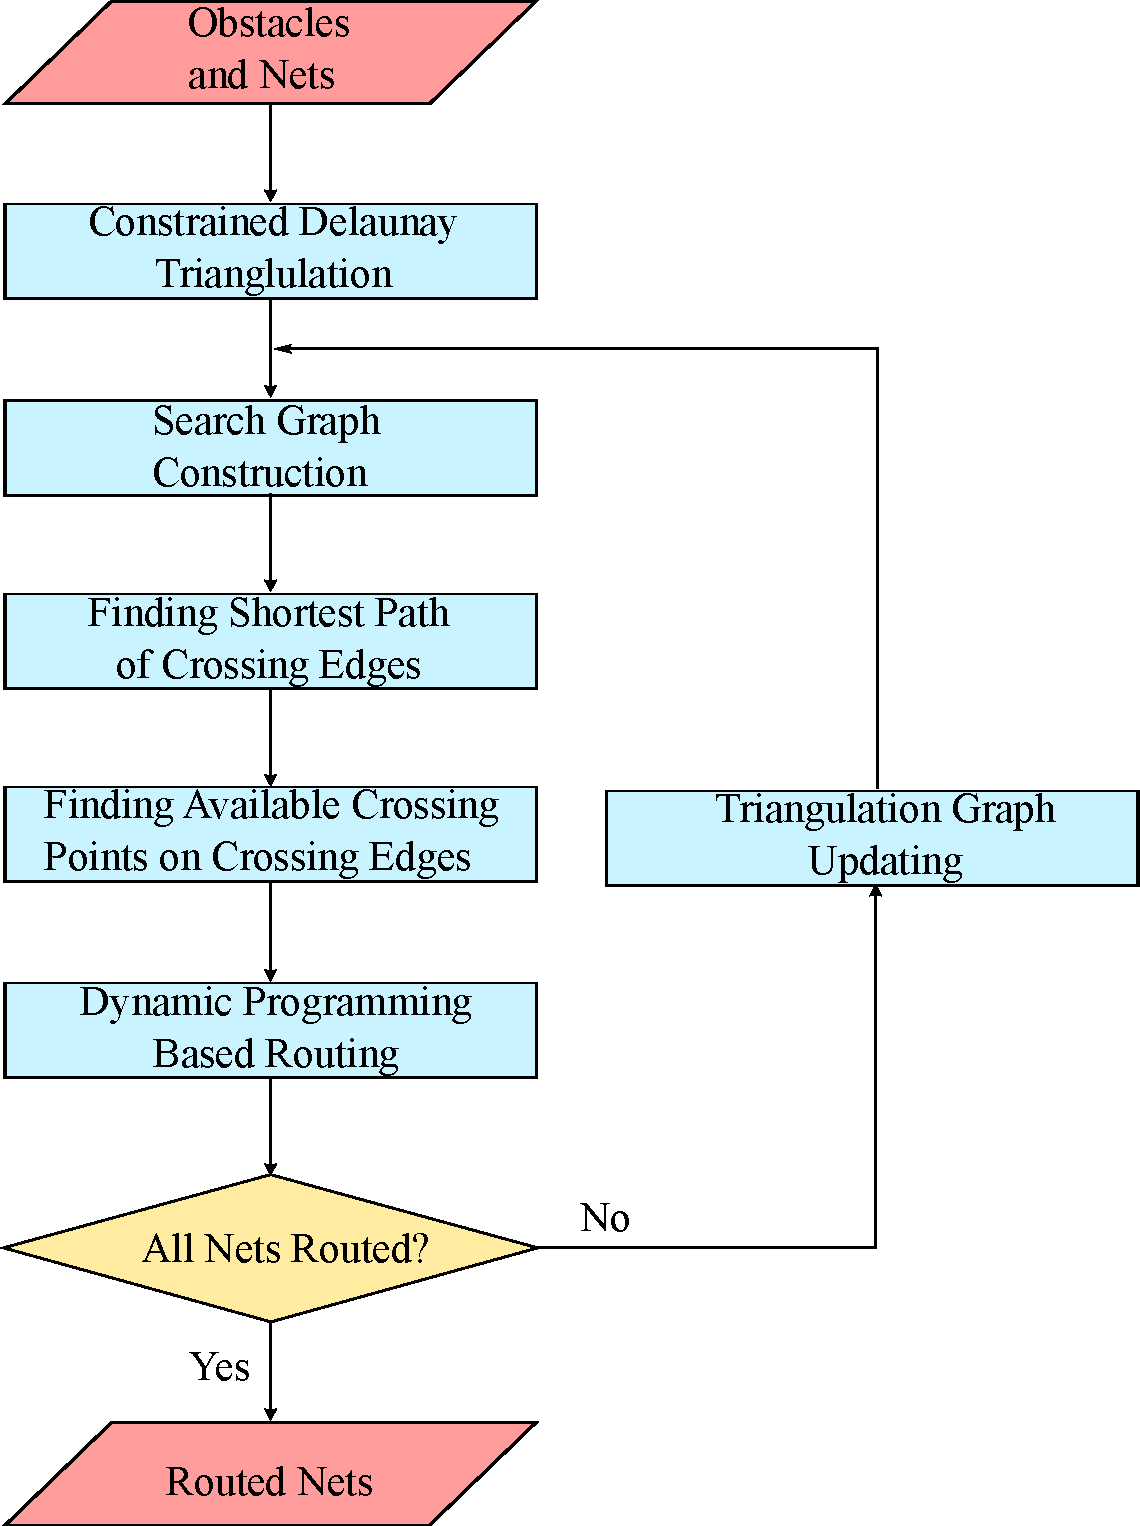
\includegraphics[width=0.9\columnwidth, angle=0]{./Figs/newFlowOpt.pdf}
\vspace{-0.2cm}
\caption{The proposed AARF routing flow.}
\label{fig:overview}
%\vspace{-0.55cm}
\end{figure}

Figure~\ref{fig:overview} shows the overall flow of the proposed any-angle router named AARF,
which is based on the Constrained Delaunay Triangulation Graph (CDT). 
Initially, the CDT is constructed on the routing terminals and routing obstacles. Then 
The flow channels for the nets are routed on the CDT one by one until all channels 
are finished. Once a flow channel is routed, the CDT will be updated accordingly. 
For each channel, the routing process consists of two steps: (1) finding a coarse routing solution, and (2) determining the physical routing channel. 
In the first step, a set of sequential CDT edges are computed by the
Dijkstra shortest path algorithm, which will be crossed by the routing channel. 
In the second step, a detailed routing algorithm based on dynamic programming is performed to find the routing channel crossing the computed CDT edges. 
As the elbows in a flow channel can severely slow down the flow rate, 
the dynamic-programming-based routing method is proposed to significantly improvement the flow rate, and thus improve the lifetime of the flow-based microfluidic biochip. 
The intrinsic idea of the dynamic-programming-based routing 
method is to assign cross points to the CDT edges of the coarse routing solution, and then optimally determine the cross points along the CDT
edges for maximized flow rate. The notations used in the paper are summarized in Table~\ref{tab:notation}.

\begin{table}[htbp]
%\scriptsize
%\small
\setlength{\tabcolsep}{1.5pt}
\renewcommand{\arraystretch}{1.2}
%\vspace{-0.20cm}
\caption{Notations used in the proposed algorithms.}
\label{tab:notation}
\centering
\vspace{-0.35cm}
\newcommand{\tabincell}[2]{\begin{tabular}{@{}#1@{}}#2\end{tabular}}
%\begin{tabular}{*{2}{|c}|}
\begin{tabular}{|c|c|}
%\begin{tabular}{p{0.9\columnwidth}}
\hline
Notations &  Meaning   \\
\hline
$N$ & Lists of input nets \\
\hline
$N_i$ & The $i^{th}$ input net \\
\hline
$V_i$ & The $i^{th}$ vertex of an input net \\
\hline
$w$ & The minimum width of channels \\
\hline
$s$ & The minimum space between channels \\
\hline
$CDT$ & Constrained Delaunay triangulation graph \\
\hline
$SG$ & Search graph \\
\hline
$Te_i$ & The $i^{th}$ triangle edge in $CDT$ \\
\hline
$T_i$ & The $i^{th}$ triangle in $CDT$ \\
\hline
$e_i$ & The $i^{th}$ neutrality edge of a triangle \\
\hline
$E$ & The set of triangle edges the routed channel crosses \\
\hline
$E_i$ & The $i^{th}$ triangle edge the routed channel crosses \\
\hline
$m$ & \tabincell{c}{The precision of dynamic programming,\\ which means the number of \\a subproblem's alternative solutions} \\
\hline
$F_{ij}$ & \tabincell{c}{The $j^{th}$ possible point of interception\\ of the routed channel and $E_i$} \\
\hline
$C_i$ & The $i^{th}$ routed channel \\
\hline
$\overline{PQ}$ & The edge between vertex $P$ and vertex $Q$ \\
\hline
$len(\overline{PQ})$ & The distance between vertex $P$ and vertex $Q$ \\
\hline
$\overline{PQR}$ & The elbow shaped by $\overline{PQ}$ and $\overline{QR}$ \\
\hline
$eqv(\overline{PQR})$ & The effective length of the turning angle of elbow $\overline{PQR}$ \\
\hline
$min\{a_1, a_2, \cdots, a_n\}$ & The smallest element among $a_1, a_2, \cdots, a_n$ \\
\hline

\end{tabular}
%\vspace{-0.45cm}
\end{table}


%\vspace{-0.1cm}
\subsection{Constrained Delaunay Triangulation Graph}
\label{sec:dtg}
%\vspace{-0.1cm}

\begin{figure}[htbp]
%%\vspace{-0.45cm}
\centering
\subfigure[]
{
\label{fig:DTGExample:a}
\begin{minipage}[b]{0.48\columnwidth}
\centering
\resizebox{\columnwidth}{!}{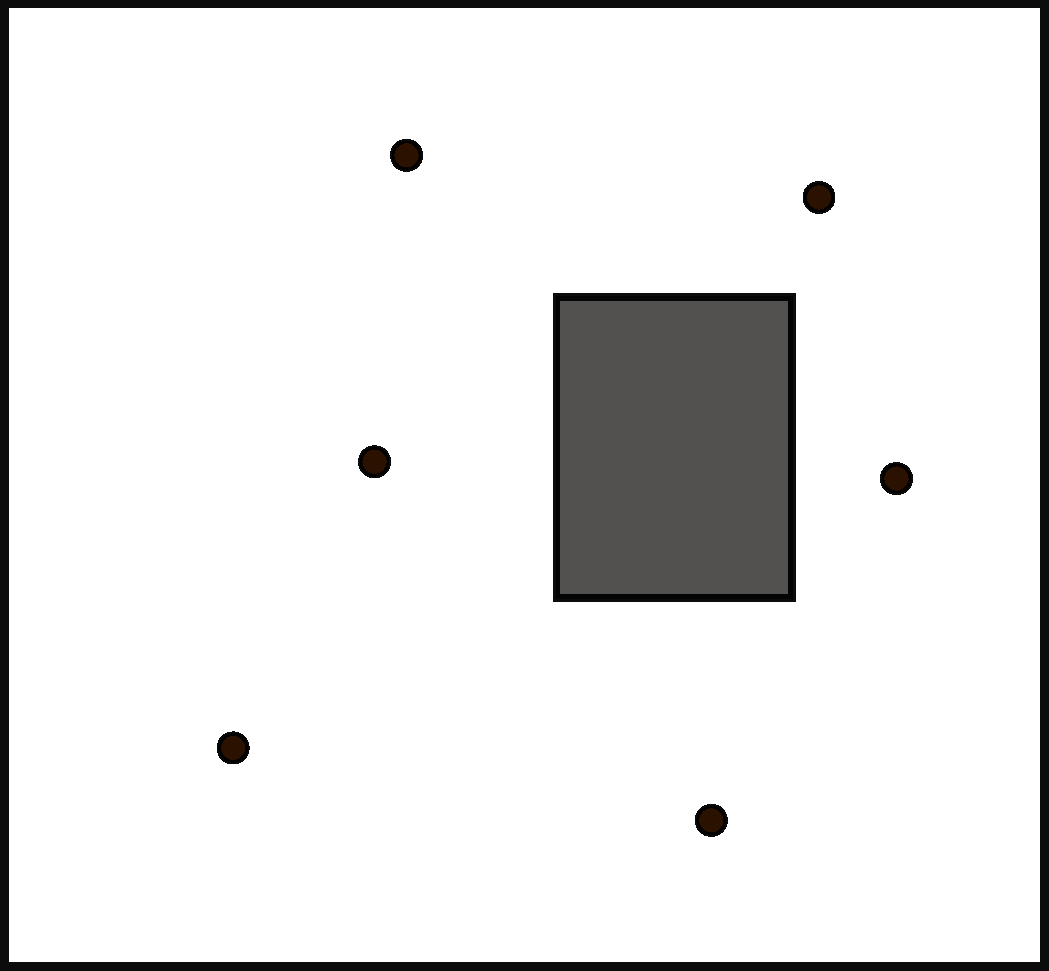
\includegraphics[width=0.48\columnwidth, angle=0]{./Figs/DTGExampleA.pdf}}
\end{minipage}%
}%
\hfil
%%\vspace{-0.25cm}
\subfigure[]
{
\label{fig:DTGExample:b}
\begin{minipage}[b]{0.48\columnwidth}
\centering
\resizebox{\columnwidth}{!}{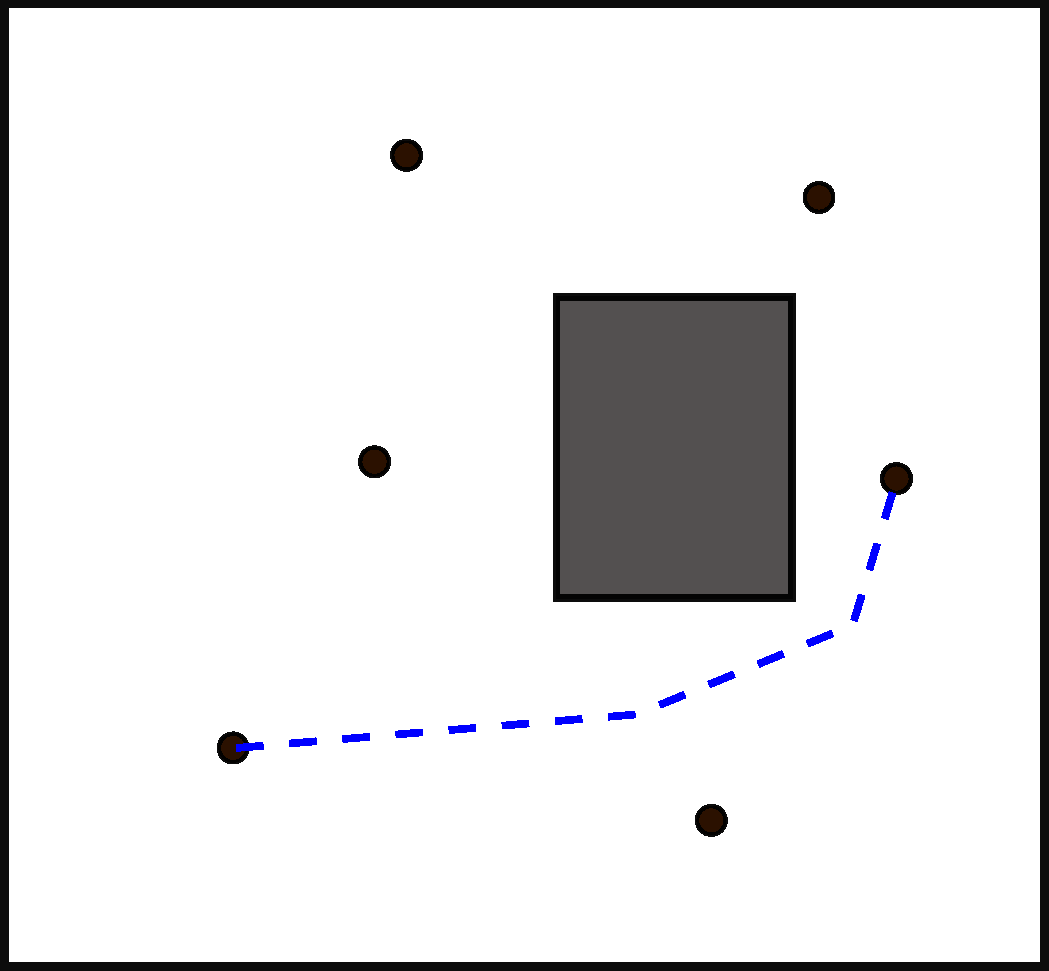
\includegraphics[width=0.48\columnwidth, angle=0]{./Figs/DTGExampleB.pdf}}
\end{minipage}%
}%
%%\vspace{-0.2cm}
\caption{Example of a non-rectilinear flow channel obtained by the any-angle routing method. (a) Input terminals and routing obstacle. (b) Any-angle routing channel.}
\label{fig:DTGExampleAB}
%%\vspace{-0.25cm}
\end{figure}

As mentioned in previous sections, the proposed any-angle routing
algorithm is based on the CDT, which consists of the {\em constrained edges}.
Here, constrained edges refer to those edges that need to be contained in the
final Delaunay triangulation result. Using the constrained Delaunay triangulation algorithm, the set of constrained edges can be specified as input. Given the routing terminals and obstacles (see Figure~\ref{fig:DTGExampleAB}), we construct the CDT as follows:

\begin{enumerate}
\item The input vertices consist of all the routing terminals, the vertices of the rectilinear routing blockages, and the vertices of the biochip's design boundary.

\item The constrained edges consist of the edges of the biochip's design boundary, as well as the edges of the routing obstacles.

\item After one round of constrained Delaunay triangulation followed by 
dynamic-programming-based routing process, the corresponding routing
 segments of the routed channel are inserted into the constrained edges, 
and the corner points between the segments are inserted into the input
 vertices.
\end{enumerate}

\begin{figure}[htbp]
%%\vspace{-0.45cm}
\centering
\subfigure[]
{
\label{fig:DTGExample:c}
\begin{minipage}[b]{0.45\columnwidth}
\centering
\resizebox{\columnwidth}{!}{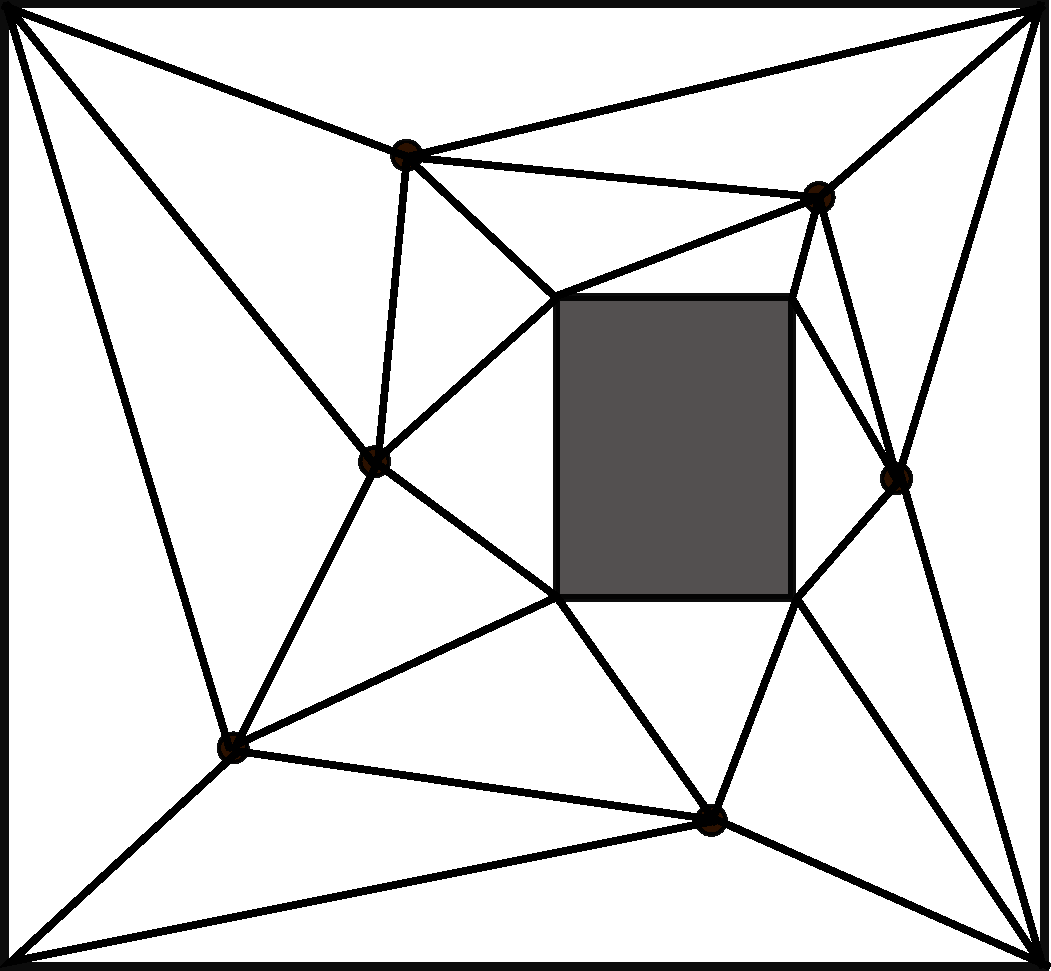
\includegraphics[width=0.8\columnwidth, angle=0]{./Figs/DTGExampleC.pdf}}
\end{minipage}%
}%
\hfil
%%\vspace{-0.25cm}
\subfigure[]
{
\label{fig:DTGExample:d}
\begin{minipage}[b]{0.45\columnwidth}
\centering
\resizebox{\columnwidth}{!}{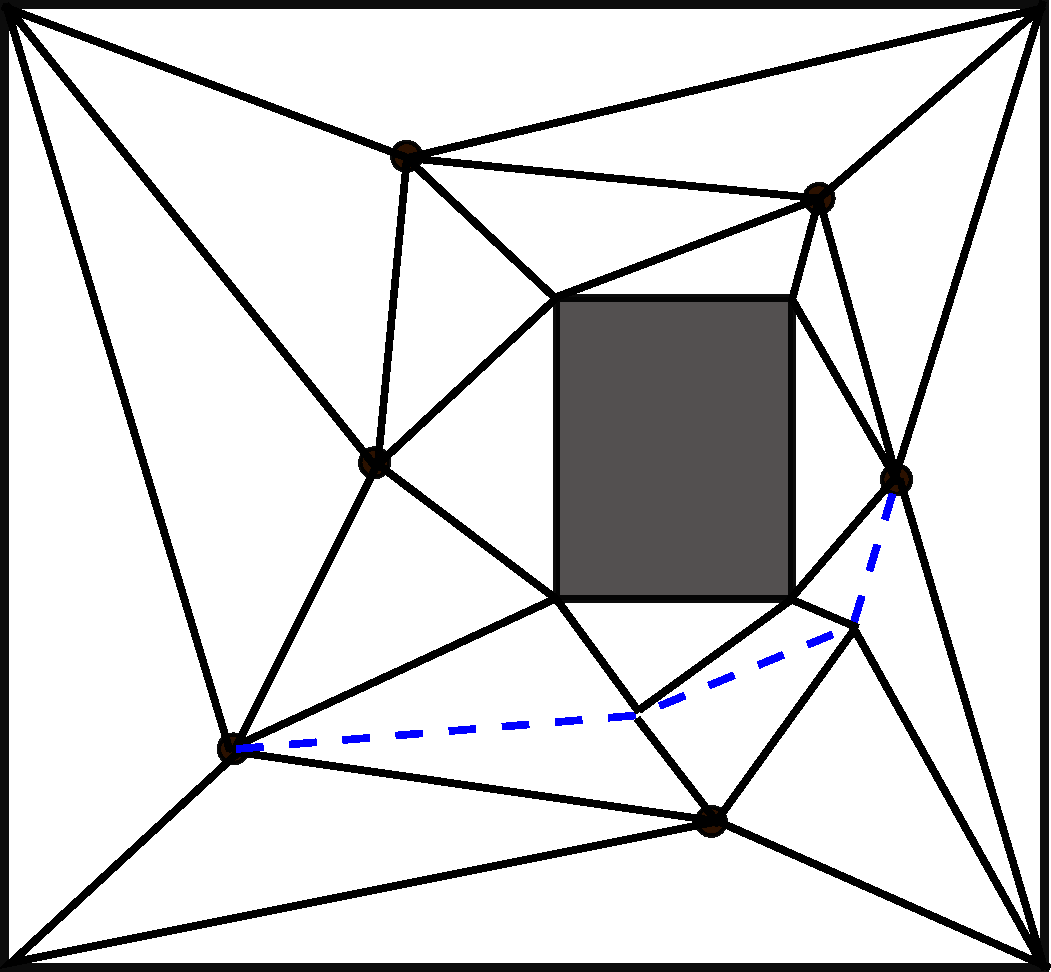
\includegraphics[width=0.4\columnwidth, angle=0]{./Figs/DTGExampleD.pdf}}
\end{minipage}%
}%
%%\vspace{-0.2cm}
\caption{Example of the constrained Delaunay triangulation graph: (a) initial constrained Delaunay triangulation graph, and (b) updated constrained Delaunay triangulation graph with a routed channel. }
\label{fig:DTGExampleCD}
%%\vspace{-0.25cm}
\end{figure}

Figure~\ref{fig:DTGExample:c} shows an example of the CDT on the initial input. And Figure~\ref{fig:DTGExample:d} shows the updated CDT with a routed flow channel. 
In Figure~\ref{fig:DTGExample:d}, all the segments of the routed flow channel are inserted into the CDT as constrained edges. 
In real biochip designs, the routing terminals are mostly located at
the boundaries of the functional modules. Here, for easily understanding
the proposed routing method, the routing terminals in the illustrating 
figures are floating, i.e., the corresponding functional modules are not 
given. We claim that the basic any-angle routing algorithm remains the same
when the routing terminals are attached to the functional modules. 
In the experiments, most routing terminals are attached to functional
modules, and the proposed routing algorithm works well. 
In the updated CDT, besides insertion of the new edges, certain edges 
in the original CDT may be removed or replaced by new edges for
incorporating the routed channel and maintaining the Delaunay Triangulation.

\subsection{Coarse Path Searching}
\label{sec:toporoute}

\begin{figure}[htbp]
%\vspace{-0.3cm}
\centering
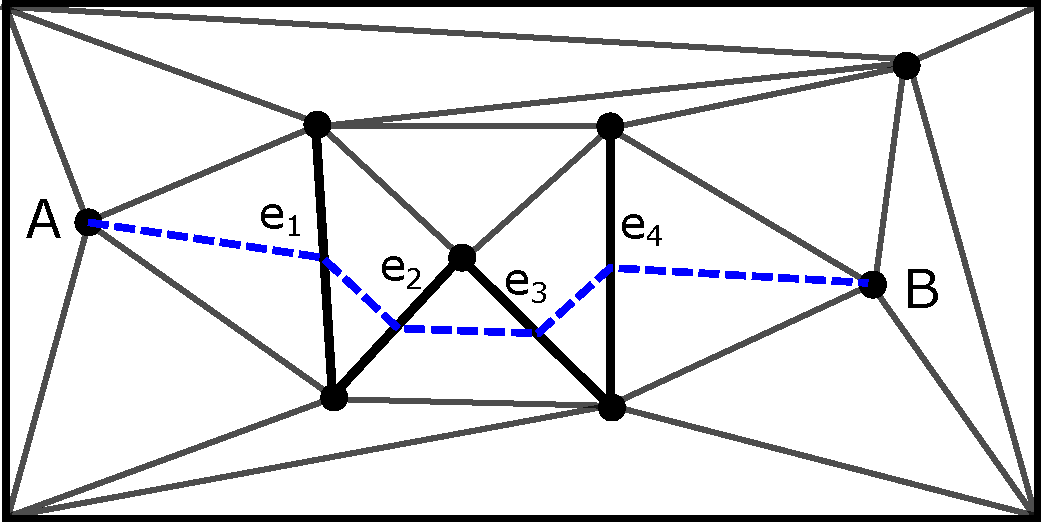
\includegraphics[width=0.75\columnwidth, angle=0]{./Figs/DTGExampleE.pdf}
\vspace{-0.15cm}
\caption{Example of coarse path searching on the CDT.}
\label{fig:DTGExampleE}
\end{figure}

After the above introduction of the CDT representation, we now describe the first step of routing, i.e., coarse routing, to search for a set of edges over the CDT edges which routing path crosses. 
After coarse routing for one net, the obtained routing solution is 
a set of sequential CDT edges. 
The flow channel to be computed should cross these edges one by one. 
To estimate the length of the routing path, we define the {\em pseudo cross point} on a CDT edge as the midpoint of the edge. 
Then the length of the coarse routing path is estimated as the sum of Euclidean distances between the source terminal and the pseudo cross point,
between the target terminal and the pseudo cross point, and between adjacent pseudo cross points. 
Figure~\ref{fig:DTGExampleE} shows an example, where the set of bold edges 
(i.e., $e_1$, $e_2$, $e_3$, and $e_4$) form the coarse routing path 
between terminals $A$ and $B$. The length of the coarse routing path 
is estimated as the total length of the dash segments. 
As shown in Figure~\ref{fig:DTGExampleE}, this routing stage 
obtains a set of CDT edges, which provides a coarse routing result. 
Therefore, in the proposed routing flow, there are two major stages: 
(1) the {\em coarse routing} stage, which obtains the coarse routing 
solution, and (2) the {\em detailed routing} stage, which computes the exact 
routing path crossing the CDT edges based on the predetermined 
coarse routing solution.

During coarse routing stage, the Dijkstra's shortest-path algorithm is performed to find the routing path.
To perform the Dijkstra's shortest-path algorithm, we define a {\em search graph} (SG), which is an undirected graph formed by the source and target terminals of the net to be routed, the midpoints of the CDT edges, the {\em neutrality edges} over the CDT (i.e., the line segments between midpoints of a triangle edges in the CDT), and certain triangle medians corresponding to source/target terminals. A search graph is constructed as follows:

\begin{enumerate}
\item The vertices of SG consist of the source and target terminal of the net to be routed, and all midpoints of all the triangle edges except those on the design's boundary, the routing blockage's boundary, and the routed channel.
 % HY: need to explain what is neutrality edge, and how design rules is violated 
\item Each neutrality edge of a triangle corresponds to an SG edge, unless it violates the design rules, or at least one terminal of the neutrality edge does not correspond to the SG vertex.
\item A triangle median should be added into SG if and only if its vertex corresponds to the source/target terminal.
\end{enumerate}


\begin{figure}[htbp]
	%%\vspace{-0.45cm}
	\centering
	\subfigure[]
	{
		\label{fig:violation:a}
		\begin{minipage}[b]{0.85\columnwidth}
			\centering
			\resizebox{\columnwidth}{!}{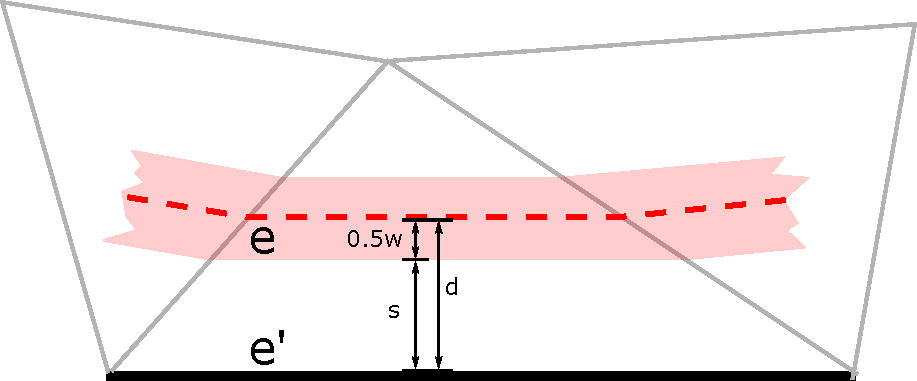
\includegraphics[width=0.85\columnwidth, angle=0]{./Figs/violationA.pdf}}
		\end{minipage}%
	}%
	\hfil
	%%\vspace{-0.25cm}
	\subfigure[]
	{
		\label{fig:violation:b}
		\begin{minipage}[b]{0.85\columnwidth}
			\centering
			\resizebox{\columnwidth}{!}{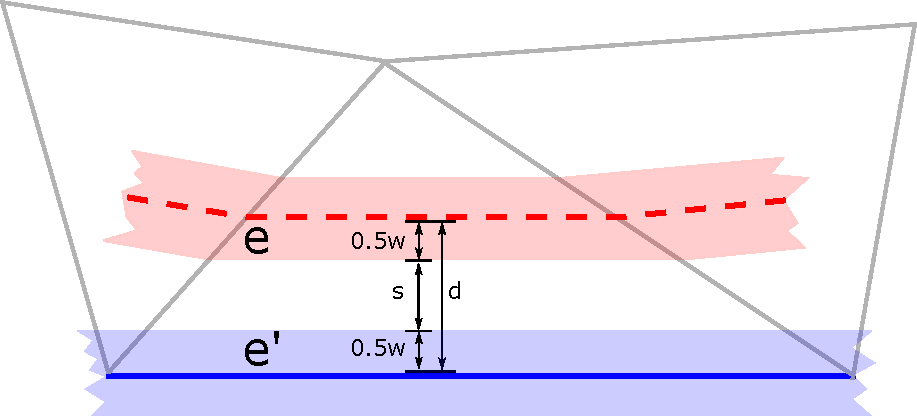
\includegraphics[width=0.85\columnwidth, angle=0]{./Figs/violationB.pdf}}
		\end{minipage}%
	}%
	\hfil
	%%\vspace{-0.2cm}
	\subfigure[]
	{
		\label{fig:violation:c}
		\begin{minipage}[b]{0.85\columnwidth}
			\centering
			\resizebox{\columnwidth}{!}{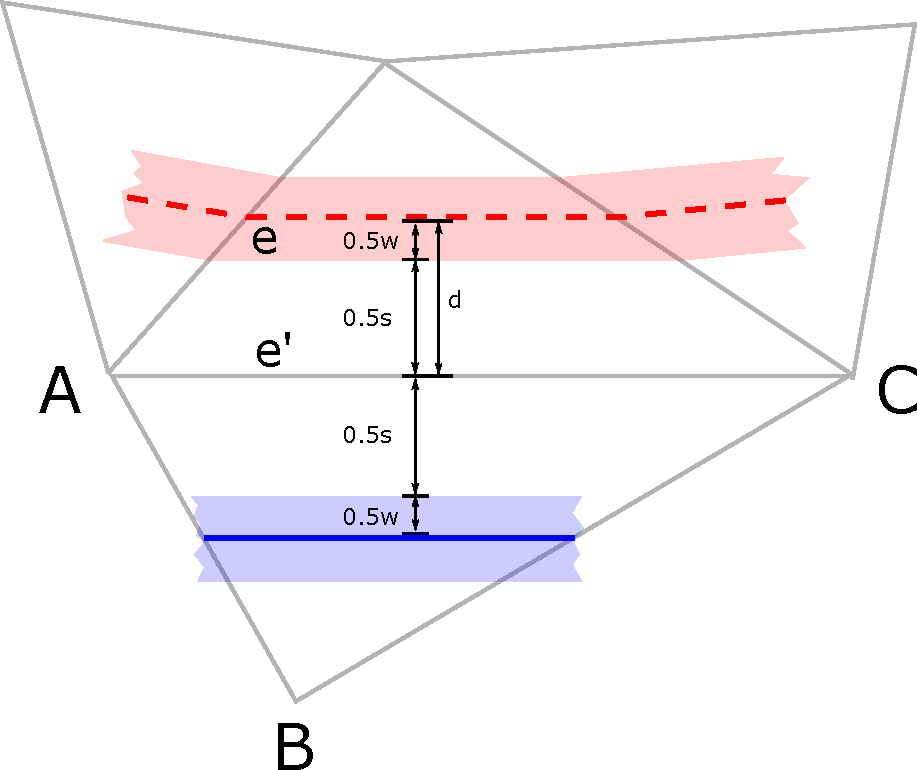
\includegraphics[width=0.85\columnwidth, angle=0]{./Figs/violationC.pdf}}
		\end{minipage}%
	}%
	\caption{Example of the design rule violation: (a) If $e$' is an edge of boundary or obstacles, $e$ breaks the design rule when $d < 0.5w+s$; (b) If $e$' is an edge of a routed channel, $e$ breaks the design rule when $d < w+s$; (c) If $e$' is a normal triangle edge, $e$ breaks design rule when $d < 0.5(w+s)$. }
	\label{fig:violation}
	%%\vspace{-0.25cm}
\end{figure}


To determine whether a neutrality edge is an edge on the search graph, 
we should verify whether it violates the design rule. 
% HY: draw a figure and explain the design rule violation according to the figure
As shown in Figure~\ref{fig:violation}, while checking neutrality edge $e$ in a triangle, there are three different cases according to the triangle edge $e$' parallel to $e$. For each case, whether $e$ breaks design rules depends on the distance $d$ between $e$ and $e$'. $e$ will be included as an edge in SG as long as the design rules are observed. 
Figure~\ref{fig:violation:a} shows the first case where $e$' is an edge of the design's boundary or obstacles. In this case, $e$ breaks the design rule if and only if $d < 0.5w+s$, where $w$ means the minimum width of channels, and $s$ means the minimum spacing between channels. By enforcing the above design rule, the spacing between the channel's boundary and the design's or obstacle's boundary is guaranteed to be not less than the required spacing $s$. 
Figure~\ref{fig:violation:b} shows the second case where $e$' is an edge from a routed channel. In this case, $e$ breaks the design rule if and only if $d < w+s$. 
Figure~\ref{fig:violation:c} shows the third case where a flow channel goes through triangle $\overline{ABC}$. Obviously, the distance between that channel and $e$ should be greater than $w+s$. Hence, $d$ is enforced to be larger than $0.5(w+s)$. 

\begin{figure}[htbp]
%\vspace{-0.3cm}
\centering
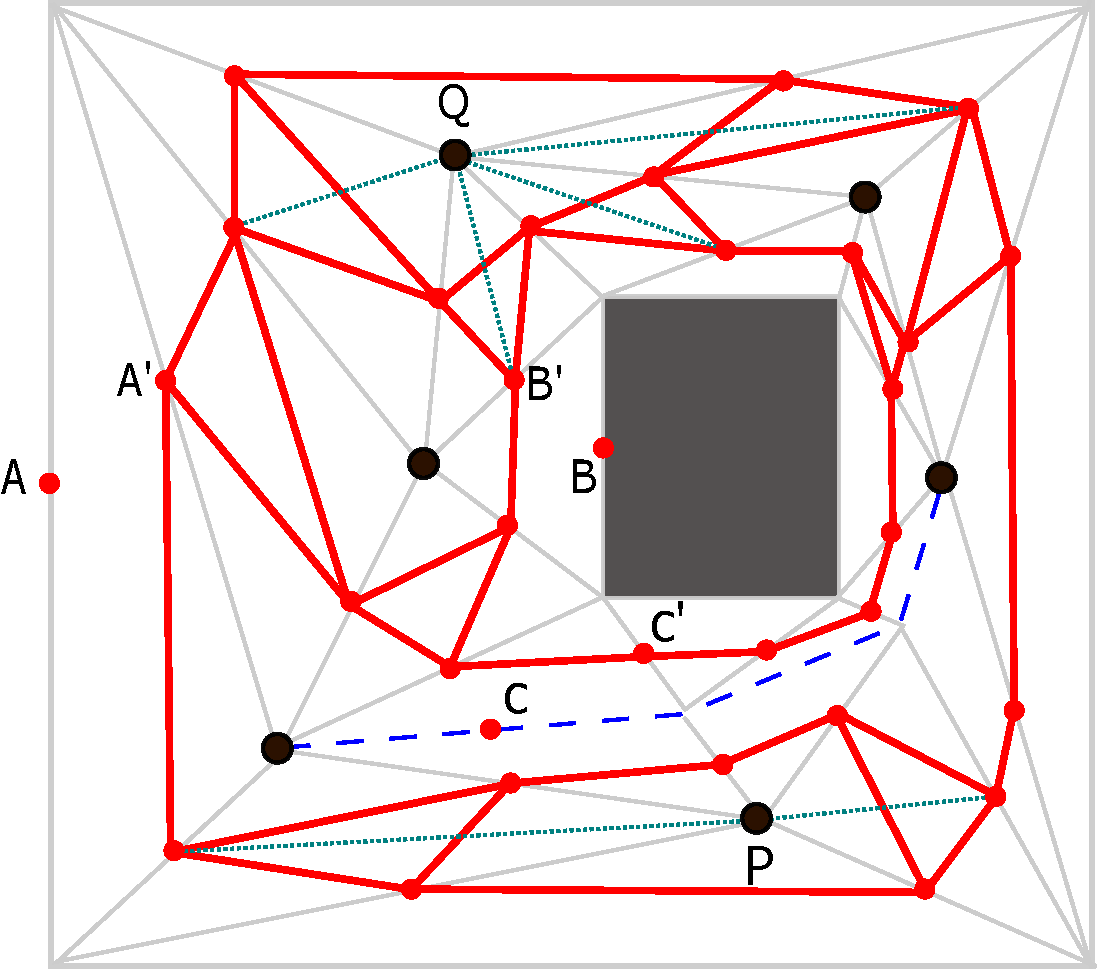
\includegraphics[width=0.9\columnwidth, angle=0]{./Figs/DTGExampleF.pdf}
\vspace{-0.15cm}
\caption{Example of the search graph.}
\label{fig:DTGExampleF}
\end{figure}


Figure~\ref{fig:DTGExampleF} shows an example of the search graph SG. 
% HY: possible to redraw this graph? emphasize the search graph
Edges in black form the CDT, and edges in red form its corresponding search graph SG. 
In Figure~\ref{fig:DTGExampleF}, points in red are midpoints of the 
triangle edges, which correspond to the vertices of SG. 
Please note that points $A$, $B$, and $C$ are not contained in SG, 
because $A$ is on the design boundary, $B$ is on the blockage boundary, 
and $C$ is on a routed flow channel. Therefore, edges $\overline{AA'}$, 
$\overline{BB'}$ and $\overline{CC'}$ are not contained in SG. 

%HY: how to give a uniform definition of SG? 

To find a shortest channel on SG, several 
additional edges connecting CDT and SG are in need because the terminals of a channel are 
triangle vertices, which are on CDT, and the segments of a channel are neutrality edges, 
which are on SG. 
Intuitively, the medians of triangles can serve as additional edges. 
When we are finding the channel between two given terminals, for example vertex $P$ and $Q$ in 
Figure~\ref{fig:DTGExampleF}, a triangle median has to be added into SG as an additional edge once its vertices include either $P$ or $Q$ (the dash line segments). Thus, we can find the shortest channel between any given pair of terminals on SG with additional edges using Dijkstra shortest path algorithm.

The result of the coarse routing stage is a path between two terminals,
 which crosses a set of triangle edges at their midpoints. 
 With the coarse routing solution, we can move on to the next routing stage, i.e., finding the detailed routing path. 
As the total effective wirelength of the coarse solution is the shortest among all possible coarse routing paths, the total effective wirelength of the detailed channel based on the coarse solution would be optimized.

%\vspace{-0.1cm}
\subsection{Dynamic-Programming-Based Detailed Routing}
\label{sec:dp}
%\vspace{-0.1cm}

\subsubsection{Crosspoint Generation on CDT Edges}

\begin{figure}[htbp]
%\vspace{-0.3cm}
\centering
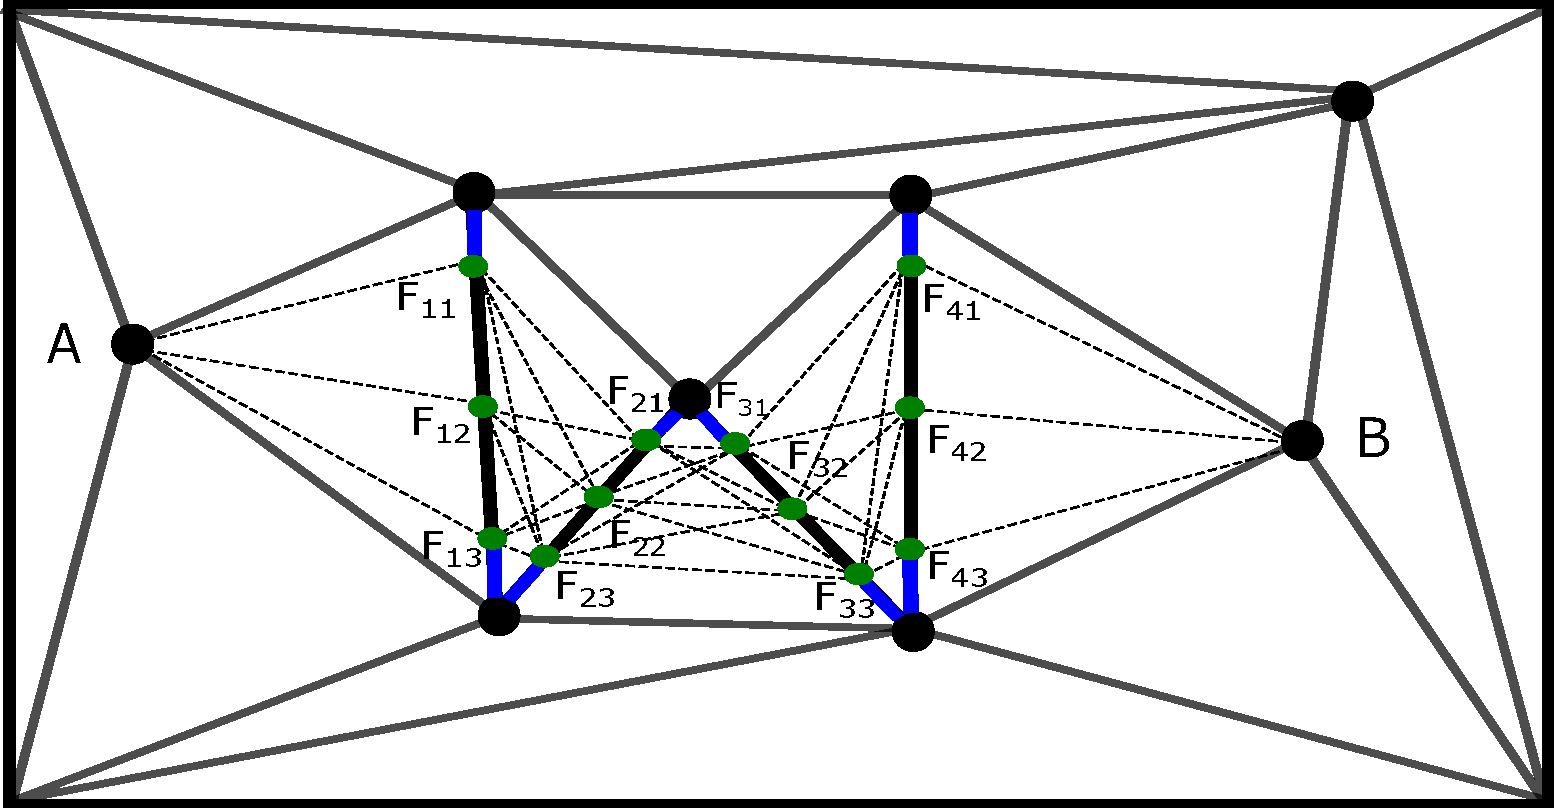
\includegraphics[width=0.9\columnwidth, angle=0]{./Figs/DP.pdf}
\vspace{-0.15cm}
\caption{Routing by dynamic programming.}
\label{fig:dp}
\end{figure}

After the coarse routing stage, a routing path is obtained which consists of a set of sequential CDT edges. 
Now we need to determine the specific crosspoints along these CDT edges. 
We propose in this paper a dynamic-programming-based detailed routing algorithm, which obtains a set of detailed routing segments connecting the given two terminals following the predetermined coarse solution. 
The proposed detailed routing algorithm guarantees optimal routing solution,
i.e., detailed routing path with minimized total effective wirelength,
along the given crosspoints on the CDT edges. 

As shown in Figure~\ref{fig:DTGExampleE}, a set of edges (bold edges in figure~\ref{fig:DTGExampleE}) is obtained after the coarse routing stage. A coarse solution which holds the length of that set of edges is denoted by the blue dashed line.
Before explaining the proposed detailed algorithm, we define a term called {\em routing pitch}, which is computed as the sum of the minimum line width and minimum line spacing. 
The routing pitch is used as the major design rule for routing the center line of the flow channels. 

Let $\{e_1, e_2, \cdots, e_n\}$ denote the CDT edges along the coarse routing solution. 
On each CDT edge, we need to identify the candidate crosspoints, where the distance between the candidate crosspoints and the CDT terminals should not be less than the routing pitch. 
As shown in Figure~\ref{fig:dp}, where the crosspoints are denoted as $F_{11}, \cdots, F_{1m}, F_{21}, \cdots, F_{2m}, \cdots, F_{n1}, \cdots, F_{nm}$,  the distance between any crosspoint (denoted by green point) and the nearest CDT terminal, which is denoted by blue segments, should satisfy the minimum spacing design rule to ensure that the distance between a crosspoint and its nearest triangle edge is not less than the routing pitch.
The actual crosspoint on the CDT edge can be either $F_{k1}, F_{km}$, or anywhere between $F_{k1}$ and $F_{km}$. 
Hence, for the given CDT edge $e_k$, the objective of the detailed routing stage is to compute the best crosspoint between $F_{k1}$ and $F_{km}$. 
Since there are infinite candidate crosspoints between $F_{k1}$ and $F_{km}$, it is difficult to compute one crosspoint for minimizing the total effective wire
length.
We propose to mark $m$ candidate crosspoints between $F_{k1}$ and $F_{km}$ (including $F_{k1}$ and $F_{km}$), and then compute the best one among them as the actual crosspoint on the CDT edge. 
When $m$ is large enough, the computed flow channel is close to the optimal solution.
Thus, the problem of finding the detailed routing path along $n$ CDT edges can be converted into $n$ subproblems, where each subproblem is corresponding to an edge.
Here, each subproblem has $m$ alternative solutions corresponding to the $m$ candidate crosspoints. 

\subsubsection{Dynamic Programming Principle}

We propose a dynamic programming algorithm to determine the actual crosspoints on the CDT edges.
Since the number of candidate crosspoints, $m$, is the key factor to determine the solution quality of the proposed dynamic programming algorithm, we define $m$ as the {\em precision of dynamic programming}. 
Before performing the dynamic programming algorithm, a {\em connection graph G(V,E)} representing all the solution space is constructed as follows: (1) The source/target terminals and all the candidate crosspoints are represented as nodes in $V$; (2) For each segment between pair of candidate crosspoints $\overline{F_{ki}F_{(k+1)j}}$ ($i,j \in [1,m]$), there is an edge $e_{kij} \in E$ between the corresponding nodes of the crosspoints; (3) For each segment between terminal-crosspoint pair, i.e., $\overline{AF_{1j}}$ between the source terminal $A$ and $F_{1j}$ (see Figure~\ref{fig:dp}), there is an edge $e_{01j} \in E$ between the corresponding nodes; (4) For each segment between crosspoint-terminal pair, i.e., $\overline{F_{nj}B}$ between crosspoint $F_{nj}$ and the target terminal $B$ (see Figure~\ref{fig:dp}), there is an edge $e_{nj1} \in E$ between the corresponding nodes. To clearly describe the dynamic programming algorithm, we define functions $f_k(i, j)$, and $g_k(r, i, j)$ as follows:


%\begin{equation}\label{eqn:dp1}
%	\begin{split}
%		f_1(i, j) = len(\overline{AF_{1j}})
%	\end{split}
%\end{equation}
%\vspace{-0.35cm}
\begin{equation}\label{eqn:dp1}
\begin{split}
g_k(r, i, j) = f_{k-1}(r, i) + len(\overline{F_{ki}F_{(k+1)j}}) + eqv(\overline{F_{(k-1)r}F_{ki}F_{(k+1)j}})
\end{split}
\end{equation}
%\vspace{-0.35cm}
\begin{equation}\label{eqn:dp1}
\begin{split}
f_k(i, j) = min\{g_k(1, i, j), g_k(2, i, j), \cdots, g_k(m, i, j)\}
\end{split}
\end{equation}
%\vspace{-0.35cm}
\noindent where $len(\overline{PQ})$ denotes the distance between $P$ and $Q$, and $eqv(\overline{PQR})$ denotes the effective length of the turning angle at point $Q$ of elbow $\overline{PQR}$. 
Each segment $\overline{F_{ki}F_{(k+1)j}}$ $(k \geq 1)$ has its precursors, denoted as $\overline{F_{(k-1)1}F_{ki}}, \overline{F_{(k-1)2}F_{ki}}, \cdots, \overline{F_{(k-1)m}F_{ki}}$.
Specially, $F_{(n+1)1}$ denotes $B$, and $F_{01}$ denotes $A$. 

%{\bf HY: errors in definition?}

%Every edge $\overline{F_{ki}F_{(k+1)j}}$ has its precursor which is one of $\overline{F_{(k-1)1}F_{ki}}, \overline{F_{(k-1)2}F_{ki}}, \cdots, \overline{F_{(k-1)m}F_{ki}}$. Specially, $F_{(n+1)1}$ is $B$ and $F_{01}$ is $A$. It is settled after we work out $f_k(i, j)$.

From the above definitions, $f_k(i, j)$ represents the shortest total effective wirelength from source terminal $A$ through $F_{(k-1)i}$ to node $F_{kj}$, and $g_k(r, i, j)$ means the sum of the length of edge $\overline{F_{ki}F_{(k+1)j}}$, the effective length of turning angle $\overline{F_{(k-1)r}F_{ki}F_{(k+1)j}}$, and the shortest total effective wirelength from source $A$ through $F_{(k-1)r}$ to $F_{ki}$. Hence, $g_k(r, i, j)$ stands for the total effective wirelength from $A$ passing through $F_{(k-1)r}$ and $F_{ki}$ and finally reaching $F_{(k+1)j}$. Every edge $\overline{F_{ki}F_{(k+1)j}}$ has its precursor which is one of $\overline{F_{(k-1)1}F_{ki}}, \overline{F_{(k-1)2}F_{ki}}, \cdots, \overline{F_{(k-1)m}F_{ki}}$. The precursor of edge $\overline{F_{ki}F_{(k+1)j}}$ is $\overline{F_{(k-1)r}F_{ki}}$ if and only if $g_k(r, i, j)$ is the shortest from $g_k(1, i, j)$ to $g_k(m, i, j)$. For example, the precursor of $\overline{F_{21}F_{34}}$ is $\overline{F_{13}F_{21}}$ if and only if $g_2(3, 1, 4)$ is the shortest among all of the $g_2(r, 1, 4)$. Specially, $f_1(i, j)$ denotes the total effective wirelength from terminal $A$ through $A$ to terminal $F_{(1)i}$. Hence, $f_1(i, j)$ equals to $len(\overline{AF_{1j}})$. With this definition, we can work out all of $f_n(1, 1), f_n(2, 1), \cdots, f_n(m, 1)$ efficiently using dynamic programming. 
Meanwhile the precursor of every edge $\overline{F_{(k-1)i}F_{kj}}$ or $\overline{F_{ni}B}$ is settled. The final step is to find one edge $\overline{F_{nr}B}$ among $\overline{F_{n1}B}, \overline{F_{n2}B}, \cdots, \overline{F_{nm}B}$, which satisfies that $f_n(r, 1)$ is the smallest among $f_n(1, 1), f_n(2, 1), \cdots, f_n(m, 1)$. After the final move, we can join $\overline{F_{nr}B}$ and its precursor $\overline{F_{(n-1)r_{n-1}}F_{nr}}$, $\overline{F_{(n-1)r_{n-1}}F_{nr}}$ and its precursor $\overline{F_{(n-2)r_{n-2}}F_{(n-1)r_{n-1}}}$, $\cdots$, and finally, $\overline{F_{1r_1}F_{2r_2}}$ and its precursor $\overline{AF_{1r_1}}$. The result is the specific channel with optimal total effective wirelength.

\section{Algorithm Detail and Complexity}
\label{sec:prca}

\subsection{Algorithm Detail}
\label{subsec:code}

\begin{algorithm2e}[h]
	\small
	%\scriptsize
	\KwIn{Net $N_i$, constrained Delaunay triangulation graph $CDT$, and the design rules.}
	\KwOut{The constructed search graph $SG$.}
	Search graph $SG = \emptyset$\;
	\ForEach{triangle edge $Te_j$ in $CDT$}{
		\If{$Te_j$ is not on design boundary, routing obstacles, or routed channels}{
			Add the midpoint of $Te_j$ into $SG$\;
		}
	}
	\ForEach{triangle $T_r$ in $CDT$}{
		\ForEach{neutrality edge $e_j$ of $T_r$}{
			\If{two terminals of $e_j$ are both included in $SG$}{
				\If{$e_j$ does not violate the design rules}{
					Add $e_j$ into $SG$\;
				}
			}
		}
	}
	\ForEach{source/target $V_j$ of net $N_i$}{
		\ForEach{triangle $T_r$ in $CDT$ that includes $V_j$}{
			\If{the midpoint $P$ of the subtense of $V_j$'s corresponding vertex is included in $SG$}{
				Add edge $\overline{V_jP}$ into $SG$\;
			}
		}
	}
	\caption{Construction of the search graph.}
	\label{alg:sg}
\end{algorithm2e}

\begin{algorithm2e}[h]
	\small
	%\scriptsize
	\KwIn{Net $N_i$, $N_i$'s corresponding source and target vertices $V_1, V_2$, the $CDT$ edge set $E$ that the coarse routing path crosses, the precision of dynamic programming $m$, and the design rules.}
	\KwOut{The routed channel $C_i$ for $N_i$.}
	\For{$j = 1$ to $|E|$}{
		Mark $m$ crosspoints from $F_{j1}$ to $F_{jm}$ on $CDT$ edge $E_j$, where the distance between any crosspoint and its nearest $CDT$ terminal satisfies the minimum spacing design rule.\;
		\If{$j > 1$}{
			\For{$k = 1$ to $m$}{
				\For{$r = 1$ to $m$}{
					Add an edge between nodes corresponding to crosspoints $F_{(j-1)r}$ and $F_{jk}$\;
				}
			}
		}
		\Else{
			\For{$k = 1$ to $m$}{
				Add an edge between nodes corresponding to source terminal $V_1$ and crosspoint $F_{jk}$\;
			}
		}
	}
	\For{$k = 1$ to $m$}{
		Add an edge between nodes corresponding to target terminal $V_2$ and crosspoint $F_{|E|k}$\;
	}
	Route net $N_i$ using dynamic programming principle\;
	\caption{Dynamic-programming-based routing.}
	\label{alg:dp}
\end{algorithm2e}

\begin{algorithm2e}[h]
\small
%\scriptsize
\KwIn{List of nets $N$ to be routed, routing obstacles $O$, the precision of dynamic programming $m$, and the design rules.}
\KwOut{The centerline of the routed flow channel for each net in $N$.}
Construct the constrained Delaunay triangulation graph $CDT$ over the given 
design boundary, obstacles' boundaries, and routing terminals\;
\For{$i = 1$ to $|N|$}
{
	Call Algorithm~\ref{alg:sg} with $N_i$ and $CDT$ as input to obtain $SG$\;
	Find the shortest path between net $N_i's$ source and vertices $V_1, V_2$ by Dijkstra's shortest path algorithm on $SG$\;
	Get the triangle edge set $E$ that the shortest path crosses\;
	Call Algorithm~\ref{alg:dp} to obtain routed channel $C_i$ with $N_i, E$ and $m$ as input\;
    \ForEach{segment $S$ of routed channel $C_i$}{
    	Add $S$ into $CDT$ as constrained edge\;
    }
}
%\For{$i = 1$ to $|N|$}{
%	Calculate the outline of channel $C_i$ according to the design rules\;
%	Remove the singularities of the outline\;
%}
\caption{Complete routing flow of AARF.}
\label{alg:aarf}
\end{algorithm2e}

Algorithm~\ref{alg:sg} shows the construction of the search graph SG. 
Initially, SG is an empty set, and the constrained Delaunay triangulation CDT is updated for the construction of the SG. 
Assume we are routing net $N_i$ whose source and target vertices are represented as $V_1$ and $V_2$, respectively.
We first add $V_1$ and $V_2$ into SG. 
For every triangle edge in CDT, we add its midpoint into SG unless the edge is on the design boundary, routing obstacles or routed channels. 
Then for each neutrality edge of the triangles in CDT, we add it into SG if the following conditions are satisfied: (1) the neutrality edge's two corresponding vertices have been included in SG, and (2) it does not violate the design rules. 
Finally, for each triangle in CDT whose vertices include $V_1$ ($V_2$), we denote the midpoint of $V_1$'s ($V_2$'s) subtense as $P$ and check the following condition. 
If $P$ already belongs to SG, we add edge $\overline{V_jP}$ into SG. 
After the above steps, the SG for net $N_i$ is constructed. 

Algorithm~\ref{alg:dp} shows the proposed dynamic-programming-based routing algorithm. 
Assume we are routing net $N_i$, and we have already obtained the coarse routing solution, i.e., a set $E$ of CDT edges that the flow channel crosses. 
For each edge $e_j$ in $E$, we mark $m$ crosspoints from $F_{j1}$ to $F_{jm}$ on the CDT edge $E_j$, where the distance between any crosspoint and its nearest CDT terminal satisfies the minimum spacing design rule. 
Then we link every pair of crosspoints $F_{(j-1)r}$ and $F_{jk}$. Specially, if $j$ equals to $1$, then we link $V_1$ and $F_{1k}$. 
Finally, for each crosspoint $F_{|E|k}$, we add an edge from $F_{|E|k}$ to the target node $V_2$. On the updated graph from these steps, we can find the detailed flow channel from $V_1$ to $V_2$ using dynamic programming algorithm as previously described.

Algorithm~\ref{alg:aarf} gives the complete flow of the proposed dynamic-programming-based any-angle routing method AARF. 
Given the input including the list of nets $N$ to be routed, the design boundary, and the routing obstacles, we first construct the constrained Delaunay triangulation graph CDT. 
All edges of obstacles or design boundary should be added into the CDT as constrained edges. 
For each net $N_i$, we first call algorithm~\ref{alg:sg} to obtain the search graph SG. 
Then we obtain the coarse routing solution on SG from source node $V_1$ of $N_i$ to its target node $V_2$ using the Dijkstra's shortest path algorithm, which is a set of triangle edges that the flow channel crosses. 
With the coarse routing solution, we call the dynamic programming algorithm~\ref{alg:dp} to obtain the detailed flow channel $C_i$ from $V_1$ to $V_2$. 
Finally, before routing the next net $N_{(i+1)}$, we insert the routed channel $C_i$ into CDT as constrained edges. 
In this way, we can route all the nets in $N$ one by one using the proposed routing algorithm.

\subsection{Complexity Analysis}
\label{complex}

Now we analyze the runtime complexity of Algorithm~\ref{alg:aarf}. 
Assume the sum of number of vertices of the design boundary, the obstacles and the routing pins is $O(M)$, a routed channel has $O(L)$ terminals in average, the number of nets is $O(N)$, and during dynamic-programming-based routing we insert $O(m)$ crosspoints on the CDT edge. 
Constructing constrained Delaunay triangulation graph takes $O(M\log(M))$ time\cite{Sloan:1993}.
Then we analyze the complexity of routing one channel. 
Suppose we have already routed $x$ flow channels. 
Thence, the total number of vertices in CDT is $O(M + xL)$, so is the number of triangle edges. 
Thus, constructing the search graph on the CDT takes $O(M + xL)$ time, 
and the search graph contains $O(M + xL)$ edges and points. 
So the Dijkstra algorithm for searching the coarse routing solution on the search graph takes $O((M + xL)^2)$ time.
Since there are $O(L)$ sub-problems corresponding to the $O(L)$ terminals on the CDT edges along the coarse routing solution, and each of them has $O(m)$ solutions, the dynamic programming stage for computing the detailed routing solution takes $O(Lm)$ time. 
Finally, we need to insert all segments of the current routed flow channel into the CDT, and this step takes $O(L(M + xL)^\frac{4}{3})$ time using the jump-and-walk approach for point location \cite{Kallmann:2004dt}. 
Nonetheless, if we reconstruct the CDT instead of inserting constrained edges, it takes $O((M + xL)\log(M + xL))$ time, which is more efficient. 
Therefore, we prefer to rebuild the CDT after each round of routing rather than directly inserting constrained edges. 
As a result, it takes $O((M + xL)^2 + Lm + (M + xL)\log(M + xL))$ time to route one channel. 
By sum of progression, our algorithm takes $O(NM^2 + N^2LM + N^3L^2 + NLm + N(M + NL)\log(M + NL))$ time. 
In most cases, $NL$ is larger than $M$ and $m$, so the overall runtime complexity is approximately $O(N^3L^2)$. 
Therefore, the longer the distance between a pair of terminals to be routed, the more crosspoints/terminals the routed channel is expected to have. And the more obstacles the chip contains, the more crosspoints the routed channel will have. Therefore, the time complexity depends mostly on the number of nets and the layout of the chip (i.e., number of obstacles, the distance between the pair of terminals in a net). Other factors, such as the precision of dynamic programming $m$, may slightly influence the runtime, but do not have any major impact.

%\vspace{-0.35cm}
\section{Experimental Results}
\label{sec:exp}
%\vspace{-0.1cm}

We have implemented the proposed AARF algorithm in C++ programming language on a 2.60GHz 32-core Intel Xeon Linux workstation with 132GB memory. 
Only a single thread is used for the experiments. 
The CGAL library is used for the implementation of the constrained Delaunay triangulation algorithm \cite{cgal}. 
A typical Manhattan routing algorithm for flow-based microfluidic biochips is tested to verify the proposed approach \cite{Yao:2015}.
 Six flow-based microfluidic biochip benchmarks are used in the experiments to verify the performance of the proposed AARF method. 
 Each benchmark has 13 to 45 flow channels to be routed. 
 Moreover, CFD simulations are performed using ANSYS Fluent to accurately verify the effectiveness and validity of our computational model to calculate the effective length of turning angles \cite{fluent}.

\begin{figure}
	%\vspace{-0.1cm}
	\label{fig:rlv}
	\centering
	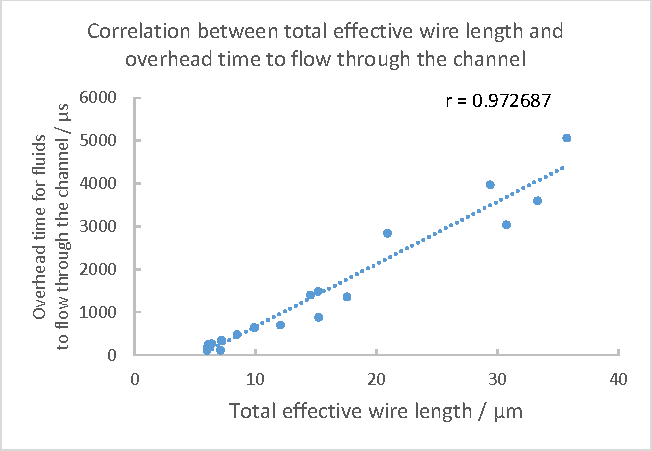
\includegraphics[width=0.9\columnwidth, angle=0]{./Figs/relativity.pdf}
	\vspace{-0.2cm}
	\caption{Computational simulation results on different total effective wirelengths of channels.}
	\label{fig:rlv}
	%\vspace{-0.55cm}
\end{figure}

\subsection{Validity Test of the Computational Model}

Our first experiment is designed to prove the validity of our computational model for simulating the flow rate in different channel conditions. 
Different turning angles affect the flow rate and hence affect the flow transmission time of fluids through the flow channel. 
The idea of converting the turning angle into effective transmission length is a classic method to evaluate the effect of different turning angles on the fluidic transmission time. 
Thus, the total effective wirelength calculated by the computational model can be used to estimate transmission time for fluids through the channel. 
In this experiment, we randomly select 20 out of total 45 channels obtained by our AARF algorithm and Manhattan routing. 
The total effective wirelength of each channel is calculated using our CFD model.
To validating the model of total effective wirelength, we obtain the flow rate of each channel through CFD simulation. 
With the flow rate from CFD simulation and the actual channel length, the transmission time of fluids through the flow channel can be accurately computed.
Figure~\ref{fig:rlv} shows the computational simulation results of the selected channels, which indicate the correlation between the transmission time and the total effective wirelength. We compute the correlation coefficient between the transmission time and the total effective wirelength as follows:

\begin{equation}
r = \frac{E(X \cdot Y) - E(X) \cdot E(Y)}{\sigma(X) \cdot \sigma(Y)}
%\vspace{-0.15cm}
\end{equation}

\noindent where $E(X)$ means the mathematical expectation of variable $X$, and $\sigma(X)$ means the standard deviation of $X$. Here, $Y$ and $X$ stand for the transmission time and the total effective wirelength, respectively. According to the computational results, the correlation coefficient is $0.97$, which verifies effectiveness of the proposed model of total effective wirelength. 
Typically, fluids spend more time flowing through a channel with longer total effective wirelength. 
Therefore, our proposed total effective wirelength model effectively estimates the impact of turning angles on fluidic transmission time.

\subsection{Effect of the CFD Model}

In the second experiment, we route all the six benchmarks with our AARF routing algorithm. 
Each benchmark is routed twice using different strategies to verify the effectiveness of the routing algorithm considering the total effective wirelength.
In strategy I, we compute the total effective wirelength considering the turning angles of elbows during routing, and find the routing solution with minimized total effective wirelength. 
In strategy II, we only minimize the channel' wirelength without considering the turning angles of elbows. 
Ideally, the total effective wirelength of strategy I should be shorter than strategy II, and the actually total wirelength may be slightly longer. 
From the previous experiment, channels with shorter total effective wirelength perform better. 
Therefore, using CFD metrics to compute the effective length of turning angles, strategy I optimizes the routing result considering the fluidic transmission time.

\begin{figure}
	%\vspace{-0.1cm}
	\label{fig:opt}
	\centering
	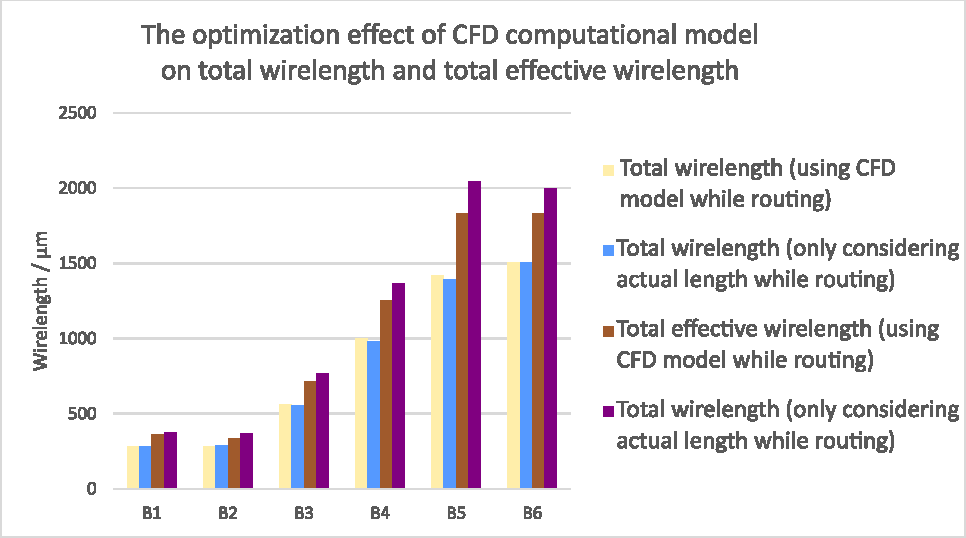
\includegraphics[width=0.95\columnwidth, angle=0]{./Figs/optimization.pdf}
	\vspace{-0.2cm}
	\caption{Comparison of two different routing methods showing the optimization of applying CFD model in routing process.}
	\label{fig:opt}
	%\vspace{-0.55cm}
\end{figure}

As shown in Figure~\ref{fig:opt}, we compute the total wirelength and total effective wirelength of each benchmark, and compare the statistics of the two routing results. 
From the figure, the total wirelengths obtained by the two routing strategies are almost the same. 
Nevertheless, the routing result obtained by strategy I has shorter total effective wirelength. 
As the total effective wirelength grows, the disparity of the two routing strategies tends to increase. 
This is because the longer a channel is, the more elbows it tends to have, with the larger solution space for optimization. 
From the results, we conclude that using our CFD model during routing can optimize the routing result, especially for biochips with long flow channels.

\begin{figure}
	%\vspace{-0.1cm}
	\label{fig:pcsc}
	\centering
	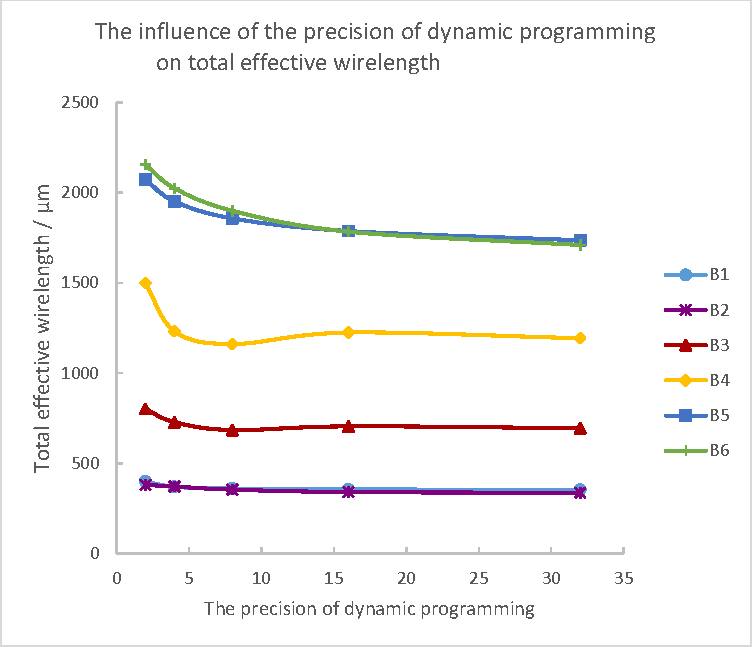
\includegraphics[width=0.95\columnwidth, angle=0]{./Figs/precision_case.pdf}
	\vspace{-0.2cm}
	\caption{Relationship between the precision of dynamic programming and the sum of total effective wirelength of one chip.}
	\label{fig:pcsc}
	%\vspace{-0.55cm}
\end{figure}

\begin{figure}
	%\vspace{-0.1cm}
	\label{fig:pcs}
	\centering
	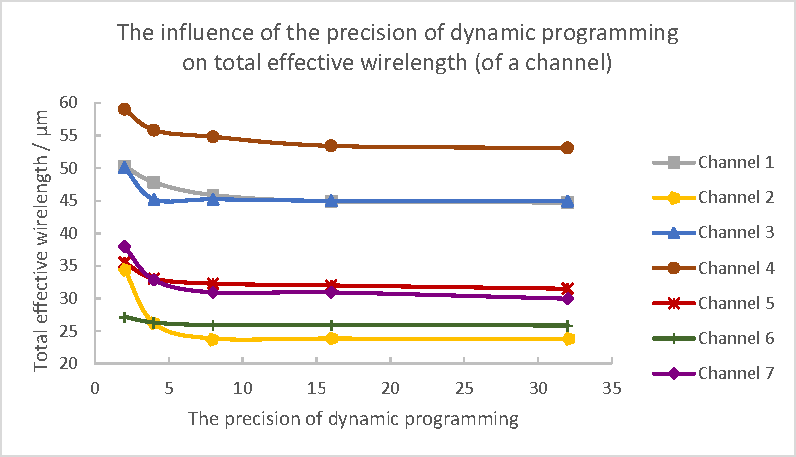
\includegraphics[width=0.95\columnwidth, angle=0]{./Figs/precision.pdf}
	\vspace{-0.2cm}
	\caption{Relationship between the precision of dynamic programming and the total effective wirelength of one specific flow channel.}
	\label{fig:pcs}
	%\vspace{-0.55cm}
\end{figure}

\subsection{Effectiveness Test of the Precision of Dynamic Programming}

In the third experiment, we test the effectiveness of the {\em precision of dynamic programming} $m$. We route each benchmark using our AARF algorithm for several times with different values of $m$. 
This experiment verifies that the proposed dynamic programming method can approach the optimal solution. 
Figure~\ref{fig:pcsc} and Figure~\ref{fig:pcs} show the experimental results. Figure~\ref{fig:pcsc} shows the relationship between the precision of dynamic programming and the sum of total effective wirelength, whereas figure~\ref{fig:pcs} shows the relationship between the precision of dynamic programming and the total effective wirelength of a specific flow channel.
Both figures show that the total effective wirelength decreases as the precision of dynamic programming grows. And the total effective wirelength tends to converge when $m$ is large enough. 
Therefore, our dynamic programming approach can practically shorten the total effective wirelength, and the routed channel approaches the optimal one when $m$ is large enough. 
Moreover, large $m$ does not severely increase the runtime.
In Figure~\ref{fig:pcsc} and ~\ref{fig:pcs}, the total effective wirelength converges when $m$ is $20$ or $30$, which is sufficiently small without significantly affecting the runtime of the overall routing algorithm.

\subsection{Comparison Between AARF and Manhattan Routing}

 \begin{table*}[htbp]
 %\scriptsize
 %\small
 \setlength{\tabcolsep}{1.5pt}
 \renewcommand{\arraystretch}{1.2}
 %\renewcommand{\arraystretch}{0.98}
 \vspace{-0.2cm}
 \caption{Routing result of Manhattan routing vs. AARF.}
 \label{tab:wocap}
 \centering
 %\vspace{-0.35cm}
 \begin{tabular}{*{15}{|c}|}
 \hline
 \raisebox{-1.4ex}[0pt]{Benchmarks} & \raisebox{-1.4ex}[0pt]{Size} & \raisebox{-1.4ex}[0pt]{\#Net} & \raisebox{-1.4ex}[0pt]{\#Block} & \raisebox{-1.4ex}[0pt]{${\cal S}_{blk}$} & \multicolumn{4}{c|}{Manhattan Routing} & \multicolumn{6}{c|}{AARF} \\
 \cline{6-15}
    & & & & & TW(${\mu}m$) & TEW(${\mu}m$) & \#Cross. & CPU(s) & TW(${\mu}m$) & $\Delta$TW & TEW(${\mu}m$) & $\Delta$TEW & \#Cross. & CPU(s)\\
 \hline
 B1 & $51 \times 58$ & 13 & 16 & 31\% & 343 & 679.136 & 0 & 0.004776 & 283.978 & 17.208\% & 360.562 & 46.909\% & 0 & 0.098981\\
 \hline
 B2 & $45 \times 63$ & 15 & 20 & 28\% & 352 & 707.909 & 0 & 0.084389 & 280.021 & 20.449\% & 335.581 & 52.595\% & 0 & 0.160829\\
 \hline
 B3 & $70 \times 73$ & 21 & 30 & 23\% & 734 & 1564.45 & 0 & 0.140010 & 562.136 & 23.415\% & 714.418 & 54.334\% & 0 & 0.577194\\
 \hline
 B4 & $84 \times 98$ & 32 & 45 & 22\% & 1330 & 2793.18 & 1 & 1.523260 & 997.754 & 24.981\% & 1253.92 & 55.108\% & 0 & 2.16655\\
 \hline
 B5 & $99 \times 113$ & 45 & 60 & 21\% & 1734 & 4100.14 & 3  & 2.510034 & 1420.47 & 18.081\% & 1833.94 & 55.271\% & 0 & 4.5973\\
 \hline
 B6 & $131 \times 130$ & 40 & 66 & 20\% & 1703 & 3983.45 & 1  & 3.016766 & 1506.74 & 11.524\% & 1831.64 & 54.019\% & 0 & 4.67568\\
 \hline
 Average & \textendash & \textendash & \textendash & \textendash & 1032.67 & 2304.71 & 0.83  & 1.21321 & 841.85 & 19.276\% & 1055.01 & 53.039\% & 0 & 2.04609\\
 \hline
 \end{tabular}
 %\vspace{-0.35cm}
 \end{table*}

Finally, we compare our AARF algorithm with a typical Manhattan routing algorithm \cite{Yao:2015}. The precision of dynamic programming is set to be 10 in this experiment. 
Table~\ref{tab:wocap} shows the details of the benchmarks, where ``Size'' represents the size of the chip, ``\#Block'' gives the number of blockages, ``\#Net'' gives the number of nets, ``${\cal S}_{blk}$'' records the percentage of the area taken by blockages, ``\#Cross.'' denotes the number of crossings on the routed chip, ``CPU'' gives the runtime of the routing algorithms in seconds, ``TW'' and ``TEW'' represent total wirelength and total effective wirelength, and ``$\Delta$TW'', ``$\Delta$TEW'' give their corresponding improvements, respectively.

From the table, the total effective wirelength of the channels routed with AARF, is $50\%$ to $58\%$ shorter than the results of Manhattan routing. 
And the total wirelength of AARF is $17\%$ to $23\%$ shorter than Manhattan routing. On average, the sum of total wirelength of all flow channels for one benchmark routed with the Manhattan routing method is $1032.67 {\mu}m$, whereas the sum decreases to $841.58 {\mu}m$ by AARF with $19.28\%$ improvement.
Moreover, the sum of total effective wirelength decreases from $2304.71 {\mu}m$ to $1055.01 {\mu}m$ when the chip is routed with AARF instead of Manhattan routing, where significant improvement of $53.04\%$ is obtained.
The comparison results denote that our any-angle routing algorithm performs much better than current Manhattan routing algorithm in terms of total wirelength and total effective wirelength, which are the most critical metrics to evaluate the performance of flow-based microfluidic biochips. 
Furthermore, our AARF algorithm avoids channel crossings since the searching algorithm is performed on the search graph, which topologically prevents the appearance of crossings. 
Nonetheless, Manhattan routing has a better performance in CPU time than AARF. On average, our AARF algorithm takes $68.85\%$ more runtime than Manhattan routing. On one hand, although the runtime for designing a single biochip is increased, the maximum runtime for all the benchmarks is still less than 5 seconds, which still guarantees the efficiency of the overall design flow. On the other hand, in the multilayer soft lithography technology, a well designed mask can be used many times for fabricating multiple biochips, which makes the design time less significant compared with the design quality and fabrication time. Therefore, considering the notable improvements in the overall solution quality, the slight runtime degradation is acceptable. 

\begin{figure}
	%\vspace{-0.1cm}
	\label{fig:mvaa}
	\centering
	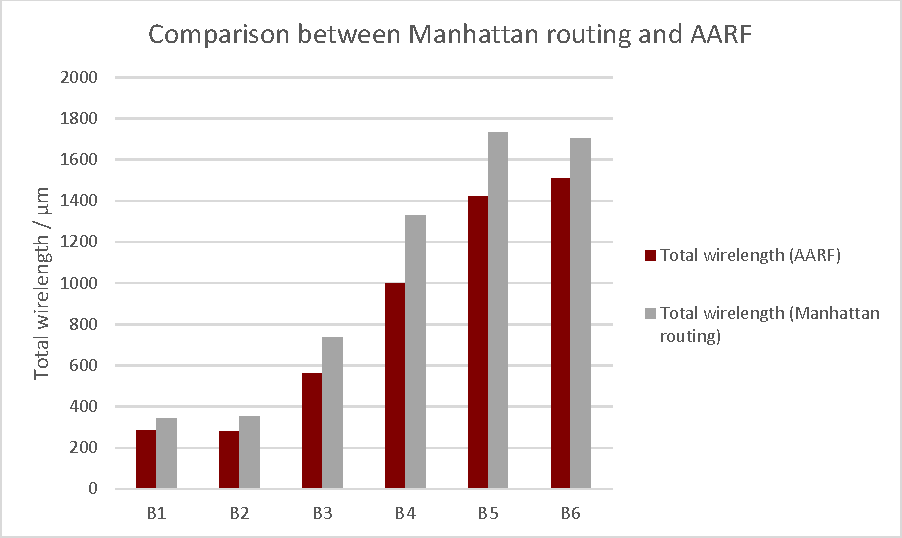
\includegraphics[width=0.95\columnwidth, angle=0]{./Figs/MR_vs_AARF_A.pdf}
	\vspace{-0.2cm}
	\caption{Comparison of the total wirelength between Manhattan routing and AARF.}
	%\vspace{-0.55cm}
	\label{fig:mvaa}
\end{figure}

\begin{figure}
	%\vspace{-0.1cm}
	\label{fig:mvab}
	\centering
	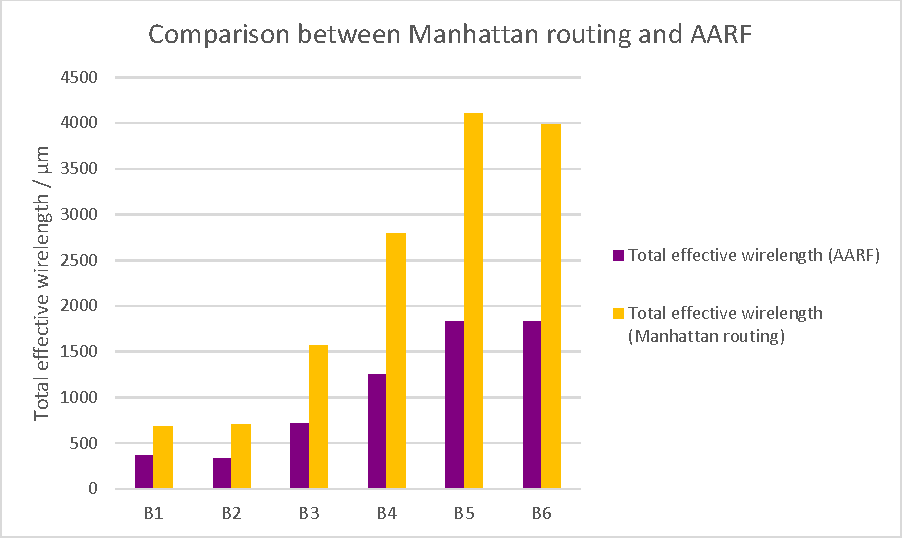
\includegraphics[width=0.95\columnwidth, angle=0]{./Figs/MR_vs_AARF_B.pdf}
	\vspace{-0.2cm}
	\caption{Comparison of the total effective wirelength between Manhattan routing and AARF.}
	%\vspace{-0.55cm}
	\label{fig:mvab}
\end{figure}

\begin{figure}[htbp]
	%%\vspace{-0.45cm}
	\centering
	\subfigure[]
	{
		%\label{fig:RC:a}
		\label{fig:b6:a}
		\begin{minipage}[b]{0.48\columnwidth}
			\centering
			\resizebox{\columnwidth}{!}{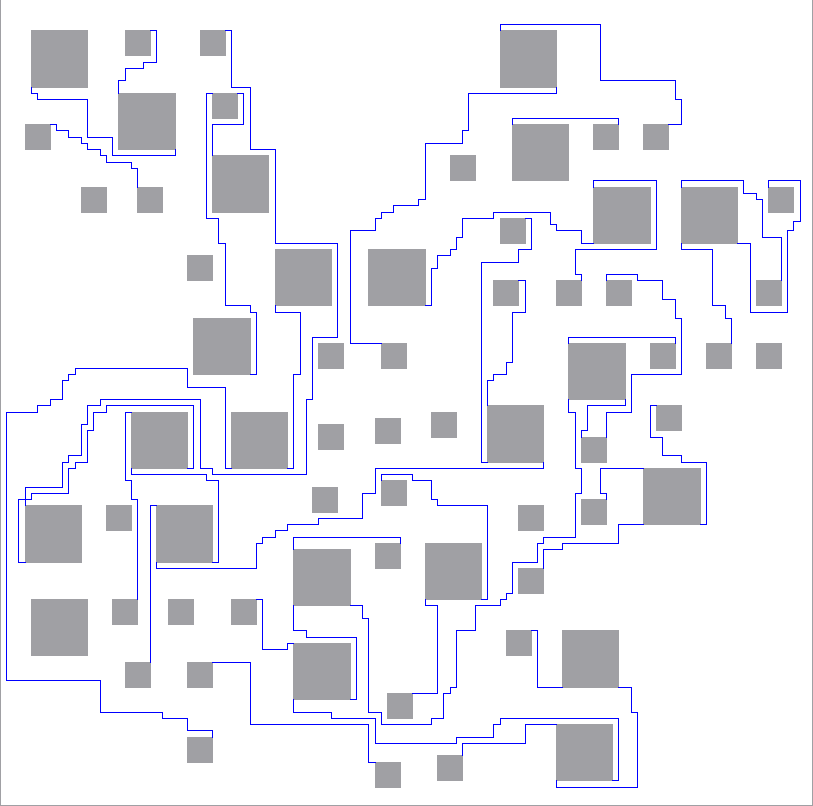
\includegraphics[width=0.48\columnwidth, angle=0]{./Figs/b6.pdf}}
		\end{minipage}%
		
	}%
	\hfil
	%%\vspace{-0.25cm}
	\subfigure[]
	{
		%\label{fig:RC:b}
		\label{fig:b6:b}
		\begin{minipage}[b]{0.48\columnwidth}
			\centering
			\resizebox{\columnwidth}{!}{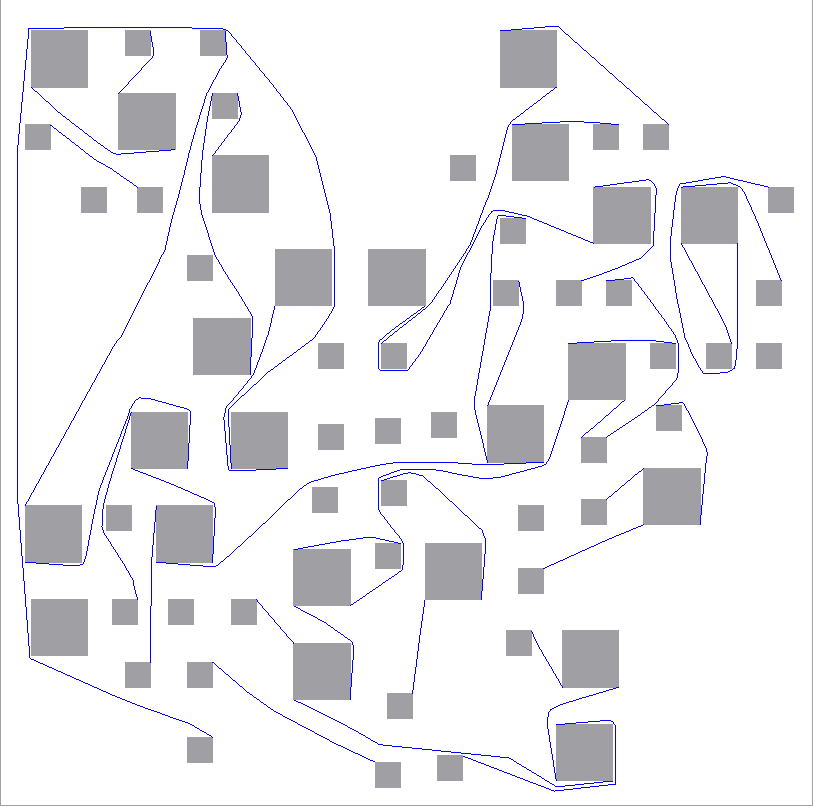
\includegraphics[width=0.48\columnwidth, angle=0]{./Figs/b6_a.pdf}}
		\end{minipage}%
	}%
	%%\vspace{-0.2cm}
	\caption{Layout of $B6$ by (a) Manhattan routing, and (b) AARF.}
	\label{fig:b6}
	%%\vspace{-0.25cm}
\end{figure}

Figure~\ref{fig:mvaa} and~\ref{fig:mvab} give the total wirelength and total effective wirelength of AARF vs. Manhattan routing, respectively. Figure~\ref{fig:b6} shows the routed layouts of benchmark $B6$ using Manhattan routing vs. AARF. From the figures, it is obvious that the total wirelength and total effective wirelength of AARF is always shorter than that of Manhattan routing. The proposed AARF algorithm obtains much better performance.

%\vspace{-0.15cm}
\section{Conclusion}
\label{sec:cln}
%\vspace{-0.1cm}

Existed automated design methods for flow-based microfluidic biochips are based on Manhattan metrics, which neglect the influence of turning angles on the flow rate and reliability. 
Those methods may not meet the requirement of assay arrival time of some timing-critical components and result in the erroneous assay outcome. 
Meanwhile, a Manhattan flow channel usually consumes extra chip area with longer wirelength. 
This paper proposed the first any-angle routing algorithm, called AARF, which is especially designed for flow-based microfluidic biochips. AARF not only incorporates the any-angle routing methodology in microfluidic biochips, but also considers effects of turning angles in the computed flow channels. To the best of our knowledge, this is the first attempt in the literature of automated design methods for flexible channel routing of flow-based microfluidic biochips.
Computational results along with CFD simulations have validated effectiveness and efficiency of AARF. 
Moreover, comparison to Manhattan routing also indicates notable improvements in both total wirelength and total effective wirelength. Our future work includes the optimization of the arithmetic operation, which further reduces the runtime of our AARF algorithm.

%\vspace{-0.25cm}
\begin{thebibliography}{99}
{
\balance 

\bibitem{Balagadde:2005bk}
F. K. Balagadde, L. You, C. L. Hansen, F. H. Arnold, and S. R. Quake, 
``Long-Term Monitoring of Bacteria Undergoing Programmed Population Control in a Microchemostat,'' 
{\em Science}, 
vol. 309, no. 5731, pp. 137-140, 2005.

\bibitem{Whitesides:2006jj}
G. M. Whitesides, 
``The Origins and the Future of Microfluidics,'' 
{\em Nature}, 
vol. 442, no. 7101, pp. 368-373, 2006.

\bibitem{Yager:2006kd}
P. Yager, T. Edwards, E. Fu, et al., %K. Helton, K. Nelson, M. R. Tam, and B. H. Weigl, 
``Microfluidic Diagnostic Technologies for Global Public Health,'' 
{\em Nature}, 
vol. 442, no. 7101, pp. 412-418, 2006.

\bibitem{Thorsen:2002ec}
T. Thorsen, S. J. Maerkl, and S. R. Quake, 
``Microfluidic Large-Scale Integration,'' 
{\em Science}, 
vol. 298, no. 5593, pp. 580-584, 2002.

\bibitem{Mark:2010fk}
D. Mark, S. Haeberle, G. Roth, et al. %F. von Stetten, and R. Zengerle, 
``Microfluidic Lab-on-a-Chip Platforms: Requirements, Characteristics and Applications,''
{\em Chemical Society Reviews},
vol. 39, no. 3, pp. 1153-1182, 2010.

\bibitem{RandM}
Research and Markets, Online Available: http://www.researchandmarkets.com/reports/2854938/microfluidic-device-system-market-global. [Accessed: Nov 10, 2016].

\bibitem{Watkins:2013id}
N. N. Watkins, U. Hassan, G. Damhorst, H. Ni, A. Vaid, W. Rodriguez, and R. Bashir,
``Microfluidic CD4+ and CD8+ T lymphocyte counters for point-of-care HIV diagnostics using whole blood,''
{\em Science Translational Medicine},
vol. 5, no. 214, p. 214ra170, 2013.


\bibitem{rice}
Rice University. ``Quick nano-bio-chip checks for oral cancer,''
{\em ScienceDaily}, www.sciencedaily.com/releases/2010/04/100405152753.htm (accessed November 10, 2016).

\bibitem{Rogers:2005vu}
J. A. Rogers and R. G. Nuzzo, 
``Recent Progress in Soft Lithography,''
{\em Materials Today}, 
vol. 8, no. 2, pp. 50-56, 2005.


\bibitem{QinRu:2016}
Q. Wang, Y. Ru, H. Yao, T.-Y. Ho, Y. Cai,
``Sequence-Pair-Based Placement and Routing for Flow-Based Microfluidic Biochips,''
{\em Proc. ASP-DAC}, 
2016, pp. 587-592.

%\bibitem{Huang:2014HX}
%X. Huang, J. Guo, X. Wang, M. Yan, Y. Kang, and H. Yu, 
%``A Contact-Imaging Based Microfluidic Cytometer with Machine-Learning for Single-Frame Super-Resolution Processing,''
%{\em PLoS One},
%2014, 9(8):e104539.

\bibitem{Studer:2004ce}
V. Studer, G. Hang, A. Pandolfi, et al., % M. Ortiz, W. F. Anderson, and S. R. Quake, 
``Scaling Properties of a Low-actuation Pressure Microfluidic Valve,'' 
{\em Journal of Applied Physics}, 
vol. 95, no. 1, pp. 393-398, 2004.

\bibitem{Minhass:2013cm}
W. H. Minhass, P. Pop, J. Madsen, and T.-Y. Ho, 
``Control Synthesis for the Flow-based Microfluidic Large-Scale Integration Biochips,''
{\em Proc. ASP-DAC}, 
%{\em Proc. Asia and South Pacific Design Automation Conference (ASP-DAC)}, 
2013, pp. 205-212.

\bibitem{Squires:2005vb}
T. M. Squires and S. R. Quake, 
``Microfluidics: Fluid Physics at the Nanoliter Scale,'' 
{\em Reviews of Modern Physics}, 
vol. 77, pp. 977-1026, 2005.

\bibitem{Unger:2000gm}
M. A. Unger, H.-P. Chou, T. Thorsen, et al., %A. Scherer, and S. R. Quake, 
``Monolithic Microfabricated Valves and Pumps by Multilayer Soft Lithography,''
{\em Science}, 
vol. 288, no. 5463, pp. 113-116, 2000.

\bibitem{Araci:2012gl}
I. E. Araci and S. R. Quake, 
``Microfluidic Very Large Scale Integration (mVLSI) with Integrated Micromechanical Valves,''
{\em Lab Chip}, 
vol. 12, no. 16, pp. 2803-2806, 2012.

%\bibitem{Untitled:wj}
%Basic Design Rules for Microfluidic Devices Fabricated at the Stanford Microfluidic Foundry. [Online]. Available: %http://web.stanford.edu/group/foundry/Basic Design Rules.html. [Accessed: 17-Aug-2014].

\bibitem{Lim:2010iq}
Y. C. Lim, A. Z. Kouzani, and W. Duan, 
``Lab-on-a-Chip: A Component View,'' 
{\em Microsystem Technologies},
vol. 16, no. 12, pp. 1995-2015, 2010.

\bibitem{Pal:2005}
R. Pal, M. Yang, R. Lin, B.N. Johnson, N. Srivastava, S.Z. Razzacki, et al., 
``An Integrated Microfluidic Device for Influenza and Other Genetic Analyses,''
{\em Lab Chip}, 
vol. 5, no. 10, pp. 1024-1032, 2005.

\bibitem{fluent}
ANSYS Fluent. [Online]. Available: http://www.ansys.com/Products/Fluids/ANSYS-Fluent/

\bibitem{Minhass:2011fh}
W. H. Minhass, P. Pop, and J. Madsen, 
``System-Level Modeling and Synthesis of Flow-Based Microfluidic Biochips,''
{\em Proc. CASE}, 
2011, pp. 225-233.

\bibitem{Minhass:2012ir}
W. H. Minhass, P. Pop, J. Madsen, and F. S. Blaga, 
``Architectural Synthesis of Flow-Based Microfluidic Large-Scale Integration Biochips,''
{\em Proc. CASE}, 2012, pp. 181-190.

%\bibitem{Melin:2006hu}
%J. Melin and S. R. Quake, 
%``Microfluidic Large-Scale Integration: the Evolution of Design Rules for Biological Automation,''
%{\em Annual Review of Biophysics and Biomolecular Structure}, 
%vol. 36, pp. 213-231, 2007.

\bibitem{SU:2004ul}
F. SU and K. Chakrabarty, 
``Architectural-Level Synthesis of Digital Microfluidics-Based Biochips,'' 
%{\em IEEE/ACM International Conference on Computer Aided Design},
{\em Proc. ICCAD},
2004, pp. 223-228.

%\bibitem{Grissom:2012gn}
%D. Grissom, K. O'Neal, B. Preciado, et al., %H. Patel, R. Doherty, N. Liao, and P. Brisk, 
%``A Digital Microfluidic Biochip Synthesis Framework,'' 
%{\em Proc. VLSI-SoC}, 
%%{\em Proc. IEEE/IFIP International Conference on VLSI and System-on-Chip (VLSI-SoC)}, 
%2012, pp. 177-182.

\bibitem{Cho:2008dk}
M. Cho and D. Z. Pan, 
``A High-Performance Droplet Routing Algorithm for Digital Microfluidic Biochips,'' 
{\em IEEE Trans. on CAD}, 
%{\em IEEE Transactions on Computer-Aided Design of Integrated Circuits and Systems}, 
vol. 27, no. 10, pp. 1714-1724, 2008.

%\bibitem{Cho:2008db}
%M. Cho and D. Z. Pan, 
%``A High-Performance Droplet Router for Digital Microfluidic Biochips,''
%{\em Proc. ISPD},
%%{\em Proc. International Symposium on Physical Design},
%2008, pp. 200-206.

\bibitem{SU:2005db}
F. SU and K. Chakrabarty, 
``Unified High-Level Synthesis and Module Placement for Defect-Tolerant Microfluidic Biochips,'' 
{\em Proc. DAC},
%{\em Proc. Design Automation Conference},
2005, pp. 825-830.

%\bibitem{SU:2006en}
%F. SU, W. Hwang, and K. Chakrabarty, 
%``Droplet Routing in the Synthesis of Digital Microfluidic Biochips,'' 
%%{\em Proc. Design, Automation and Test in Europe},
%{\em Proc. DATE},
%2006, vol. 1, pp. 1-6.

%\bibitem{Xu:2007fz}
%T. Xu and K. Chakrabarty, 
%``Integrated Droplet Routing in the Synthesis of Microfluidic Biochips,'' 
%{\em Proc. DAC},
%%{\em Proc. Design Automation Conference},
%2007, pp. 948-953.

\bibitem{Yuh:2007kd}
P.-H. Yuh, C.-L. Yang, and Y.-W. Chang, 
``Placement of Defect-Tolerant Digital Microfluidic Biochips Using the T-Tree Formulation,''
{\em ACM JETC}, 
vol. 3, no. 3, Artical No. 13, 2007.

%\bibitem{Yuh:2008gh}
%P.-H. Yuh, C.-L. Yang, and Y.-W. Chang, 
%``BioRoute: A Network-Flow-Based Routing Algorithm for the Synthesis of Digital Microfluidic Biochips,'' 
%{\em IEEE Trans. on CAD}, 
%%{\em IEEE Transactions on Computer-Aided Design of Integrated Circuits and Systems}, 
%vol. 27, no. 11, pp. 1928-1941, 2008.

\bibitem{Huang:2011iy}
T.-W. Huang and T.-Y. Ho, 
``A Two-Stage Integer Linear Programming-Based Droplet Routing Algorithm for Pin-Constrained Digital Microfluidic Biochips,''
{\em IEEE Trans. on CAD}, 
%{\em IEEE Transactions on Computer-Aided Design of Integrated Circuits and Systems}, 
vol. 30, no. 2, pp. 215-228, 2011.

%\bibitem{Yuh:2009gk}
%P.-H. Yuh, S. S. Sapatnekar, C.-L. Yang, and Y.-W. Chang, 
%``A Progressive-ILP-Based Routing Algorithm for the Synthesis of Cross-Referencing Biochips,'' 
%{\em IEEE Trans. on CAD}, 
%%{\em IEEE Transactions on Computer-Aided Design of Integrated Circuits and Systems}, 
%vol. 28, no. 9, pp. 1295-1306, 2009.

%\bibitem{Xiao:2010cr}
%Z. Xiao and E. F. Y. Young, 
%``CrossRouter: A Droplet Router for Cross-Referencing Digital Microfluidic Biochips,''
%{\em Proc. ASP-DAC}, 
%%{\em Proc. Asia and South Pacific Design Automation Conference (ASP-DAC)}, 
%2010, pp. 269-274.

%\bibitem{Wang:2014wq}
%Q. Wang, Y. Shen, H. Yao, T.-Y. Ho, and Y. Cai, 
%``Practical Functional and Washing Droplet Routing for Cross-Contamination Avoidance in Digital Microfluidic %Biochips,''
%{\em Proc. DAC}, 
%%{\em Proc. Design Automation Conference (DAC)}, 
%2014, pp. 1-6.

\bibitem{Minhass:2012th}
W. H. Minhass, P. Pop, and J. Madsen, 
``Synthesis of Biochemical Applications on Flow-Based Microfluidic Biochips Using Constraint Programming,''
{\em Proc. DTIP},
2012 , pp. 37-41.


\bibitem{Lin:2014ex}
C.-X. Lin, C.-H. Liu, I.-C. Chen, D. T. Lee, and T.-Y. Ho,
``An Efficient Bi-criteria Flow Channel Routing Algorithm for Flow-Based Microfluidic Biochips,''
{\em Proc. DAC},
%{\em Proc. Design Automation Conference},
2014, pp. 1-6.

\bibitem{Amin:2009eh}
N. Amin, W. Thies, and S. Amarasinghe, 
``Computer-Aided Design for Microfluidic Chips Based on Multilayer Soft Lithography,''
{\em Proc. ICCD}, 
%{\em Proc. IEEE International Conference on Computer Design}, 
2009, pp. 2-9.

\bibitem{Hu:2014dt}
K. Hu, T. A. Dinh, T.-Y. Ho, and K. Chakrabarty, 
``Control-Layer Optimization for Flow-Based mVLSI Microfluidic Biochips,''
{\em Proc. CASE}, Article No. 16, 2014.

\bibitem{Yao:2015}
H. Yao, T.-Y. Ho, and Y. Cai, 
``PACOR: practical control-layer routing flow with length-matching constraint for flow-based microfluidic biochips,'' 
{\em Proc. DAC},
%{\em Proc. Design Automation Conference},
2015, pp. 1-6.

\bibitem{wq:2016}
Q. Wang, Y. Ru, H. Yao, T.-Y. Ho, and Y. Cai,
``Sequence-pair-based Placement and Routing for Flow-based Microfluidic Biochips,''
{\em Proc. of ASP-DAC},
2016, pp. 587-592.


\bibitem{Sloan:1993}
S. W. SLOAN, 
``A Fast Algorithm for Generating Constrained Delaunay Triangulations,''
{\em Computers \& Structures}, 
%{\em Proc. IEEE International Conference on Computer Design}, 
vol. 47, no. 3, pp. 441-450, 1993.

\bibitem{Kallmann:2004dt}
Marcelo Kallmann, Hanspeter Bieri, and Daniel Thalmann, 
``Fully Dynamic Constrained Delaunay Triangulations,''
{\em Geometric Modeling for Scientific Visualization}, 
Springer, pp. 241-257, 2004.

\bibitem{cgal}
The Computational Geometry Algorithms Library. http://www.cgal.org/.


% \bibitem{Chao:1992fm}
% T.-H. Chao, Y.-C. Hsu, J.-M. Ho, and A. B. Kahng, 
% ``Zero Skew Clock Routing with Minimum Wirelength,''
% {\em IEEE Trans. on Circuits and Systems II}, 
% %{\em IEEE Transactions on Circuits and Systems II: Analog and Digital Signal Processing}, 
% vol. 39, no. 11, pp. 799-814, 1992.

%\bibitem{Cong1999}
%J. Cong, A. B. Kahng, C.-K. Koh, and C.-W. Albert Tsao,
%``Bounded-Skew Clock and Steiner Routing,''
%{\em ACM Transactions on Design Automation of Electronic Systems}, Vol. 3, No. 3, 1998, pp. 341–388.

% \bibitem{Alidaee:2006kf}
% B. Alidaee, F. Glover, G. Kochenberger, and H. Wang, 
% ``Solving the Maximum Edge Weight Clique Problem via Unconstrained Quadratic Programming,''
% {\em European Journal of Operational Research}, 
% vol. 181, no. 2, pp. 592-597, 2006.

% \bibitem{Hart:1968bf}
% P. E. Hart, N. J. Nilsson, and B. Raphael, 
% ``A Formal Basis for the Heuristic Determination of Minimum Cost Paths,''
% {\em IEEE Trans. on Systems Science and Cybernetics}, 
% %{\em IEEE Transactions on Systems Science and Cybernetics}, 
% vol. 4, no. 2, pp. 100-107, 1968.

% \bibitem{McMurchie:1995hs}
% L. McMurchie and C. Ebeling, 
% ``PathFinder: A Negotiation-Based Performance-Driven Router for FPGAs,''
% {\em Proc. ACM Symposium on Field-Programmable Gate Arrays},
% 1995, pp. 111-117.

%\bibitem{Papadimitriou:1981gb}
%C. H. Papadimitriou, 
%``On the Complexity of Integer Programming,''
%{\em Journal of the ACM}, 
%vol. 28, no. 4, pp. 765-768, 1981.


% %\vspace{-0.005in}
% \bibitem{gurobi}
% Gurobi Optimizer. http://www.gurobi.com/.

% %\vspace{-0.005in}
% \bibitem{Garey79}
% M. R. Garey, D. S. Johnson, 
% ``Computers and Intractability: A Guide to the Theory of NP-completeness'',
% Freeman, New York, 1979, pp. 53-56.

%\bibitem{networkflow}
%R. K. Ahuja, T. L. Magnanti, and J. B. Orlin, 
%Network Flows: Theory, Algorithms, and Applications, Prentice Hall, 1993, p. 318.

}
\end{thebibliography}
\newpage
\vspace{-0.90cm}
\begin{IEEEbiography}[{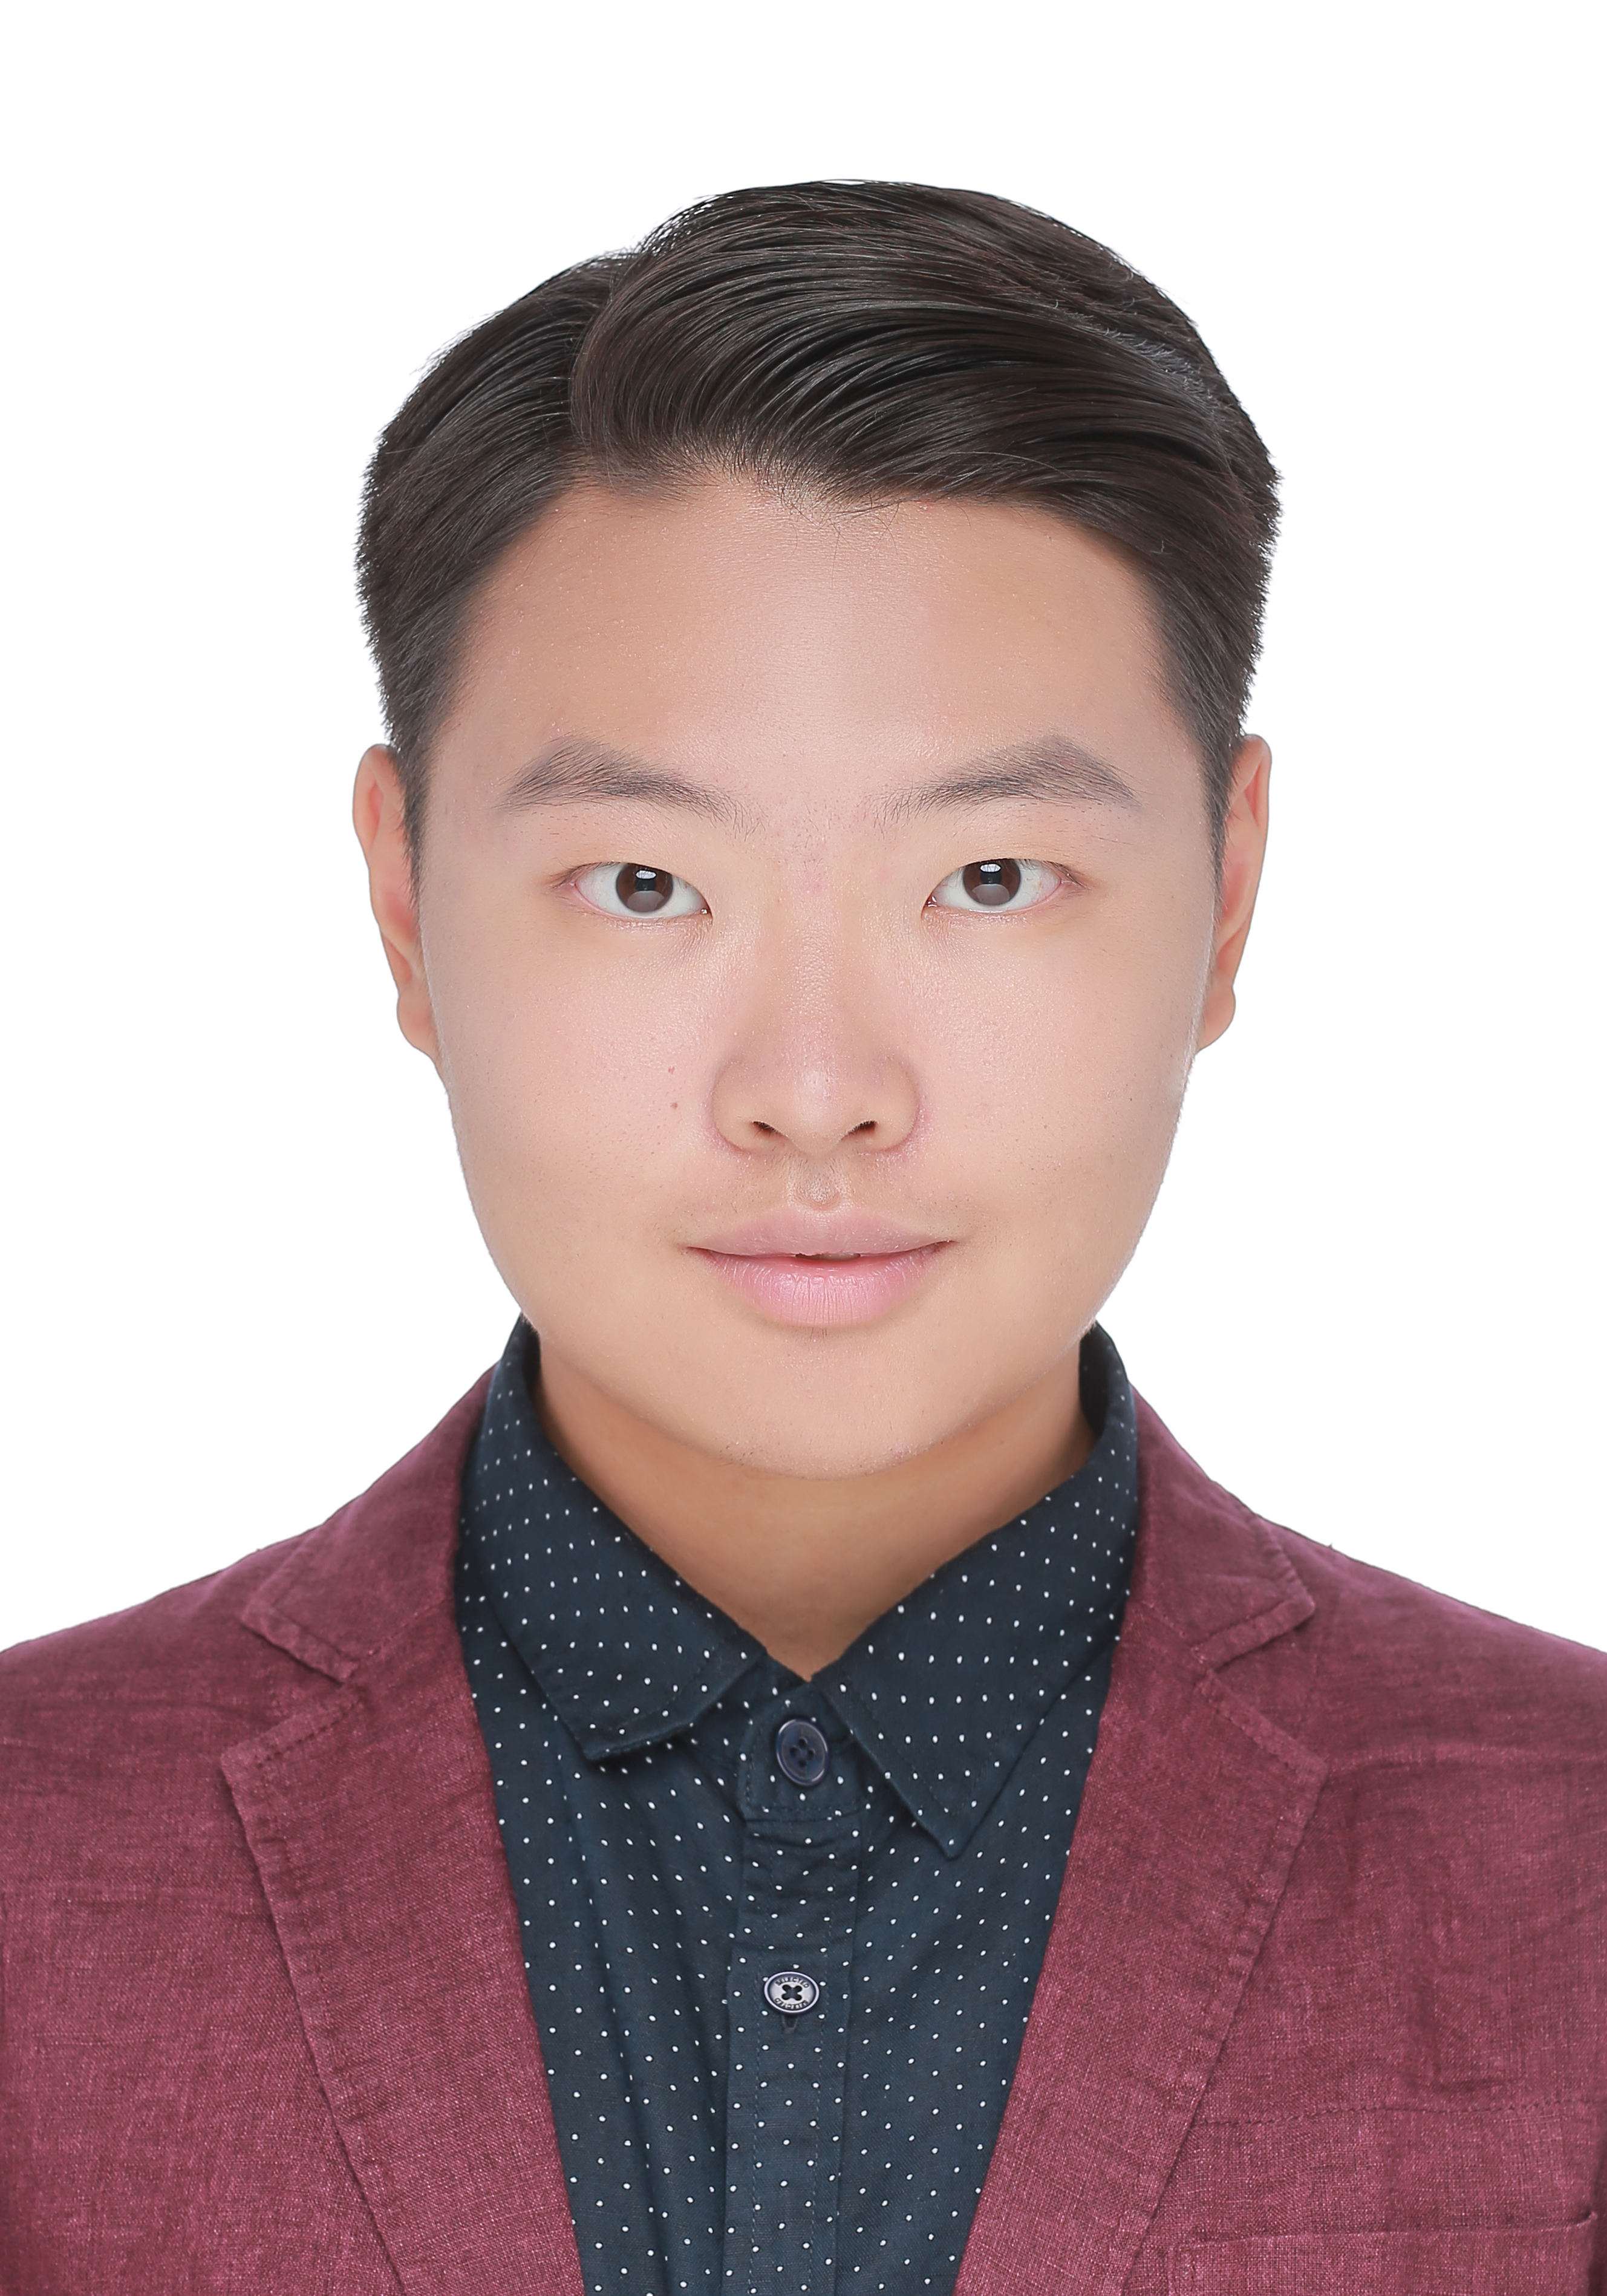
\includegraphics[width=1in,height=1.25in,clip,keepaspectratio]{./photo/ykl.jpg}}]{Kailin Yang}  is currently an undergraduate student in the Department of Computer Science and Technology, Tsinghua University, Beijing, China.
\end{IEEEbiography}

\begin{IEEEbiography}[{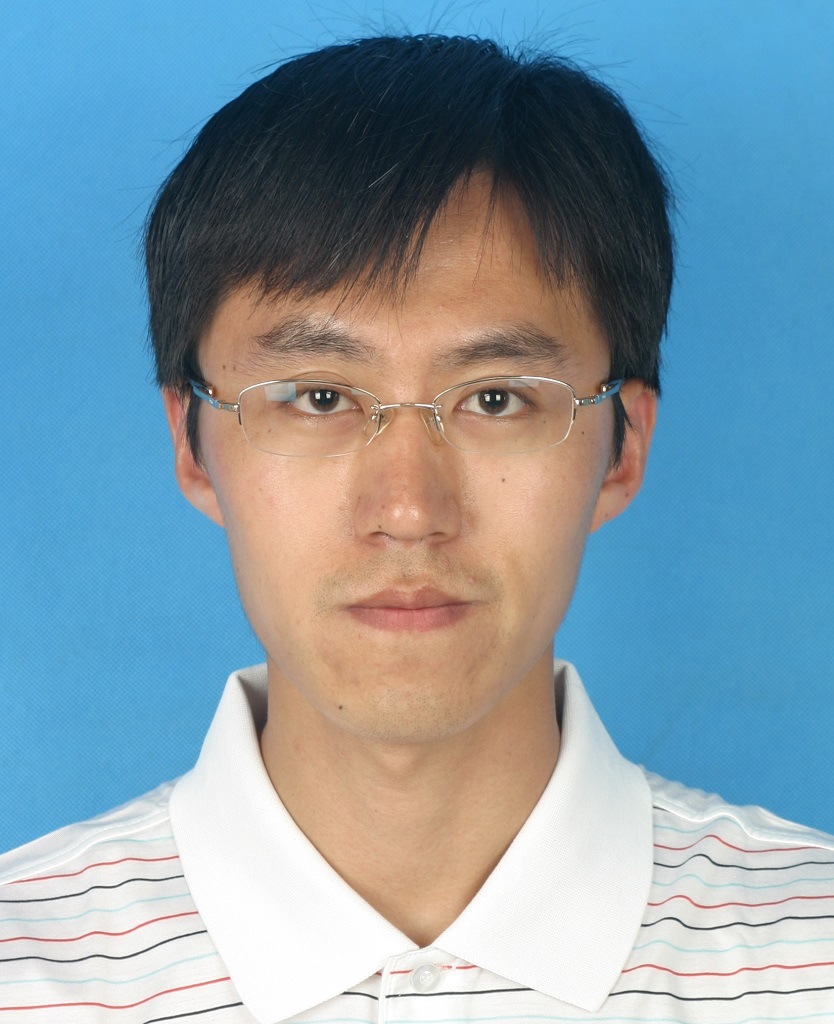
\includegraphics[width=1in,height=1.25in,clip,keepaspectratio]{./photo/hy.jpg}}]{Hailong Yao (SM'15)} received the B.S. degree 
in computer science and technology from Tianjin University, Tianjin, 
China, in 2002, and the Ph.D. degree in computer science 
and technology from Tsinghua University, Beijing, China, in 2007. 
From 2007 to 2009, he was a postdoctoral research 
scholar in the Department of Computer Science and Engineering, 
University of California at San Diego, La Jolla. He joined the 
Department of Computer Science and Technology in Tsinghua University 
as an assistant professor in September 2009. 
His research interests include computer-aided design for microfluidic biochips, very large scale integration (VLSI) physical design, design-manufacturing interface, analog routing, etc. Dr. Yao has published over 40 research papers. He received two Best Paper Award Nominations at ICCAD in 2006 and 2008, respectively. He received the ISQED Best Paper Award Nomination in 2011.
\end{IEEEbiography}


\vspace{-0.90cm}
\begin{IEEEbiography}[{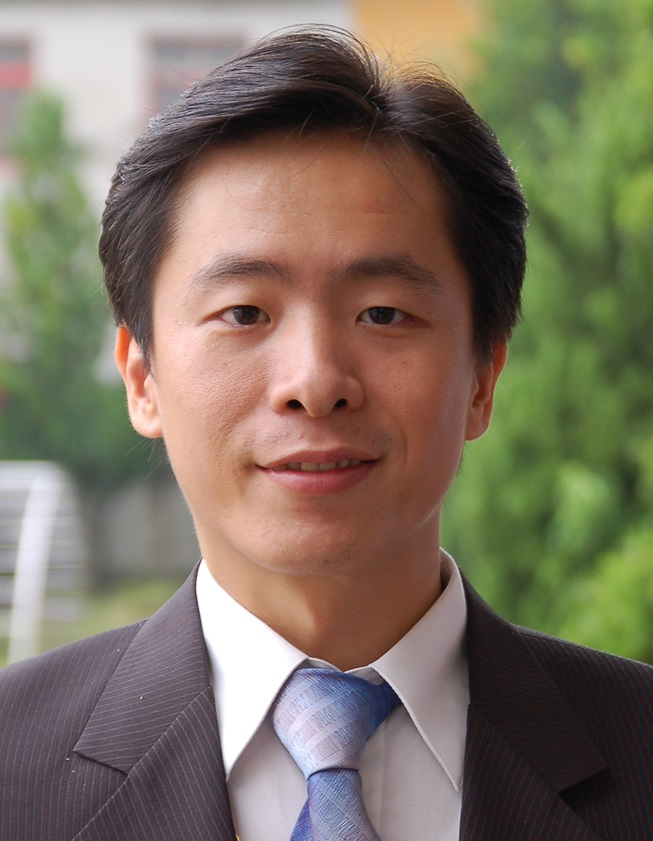
\includegraphics[width=1in,height=1.25in,clip,keepaspectratio]{./photo/T-YHo.jpg}}]{Tsung-Yi Ho (SM'12)} received his Ph.D. in Electrical Engineering from National Taiwan University in 2005. He is a Professor with the Department of Computer Science of National Tsing Hua University, Hsinchu, Taiwan. From 2007 to 2014 and 2015, he was with National Cheng Kung University and National Chiao Tung University, respectively. His research interests include design automation and test for microfluidic biochips and nanometer integrated circuits. He has presented 10 tutorials and contributed 10 special sessions in ACM/IEEE conferences, all in design automation for microfluidic biochips. He was a recipient of the Best Paper Awards at the VLSI Test Symposium (VTS) in 2013 and IEEE Transactions on Computer-Aided Design of Integrated Circuits and Systems in 2015. He currently serves as an ACM Distinguished Speaker, a Distinguished Lecturer of the IEEE CAS Society, the Chair of the IEEE Computer Society Tainan Chapter, the Chair of the ACM SIGDA Taiwan Chapter, and Associate Editor of the ACM Journal on Emerging Technologies in Computing Systems, ACM Transactions on Design Automation of Electronic Systems, IEEE Transactions on Computer-Aided Design of Integrated Circuits and Systems, IEEE Transactions on Very Large Scale Integration Systems, Guest Editor of IEEE Design \& Test of Computers.
\end{IEEEbiography}

\vspace{-0.90cm}
\begin{IEEEbiography}[{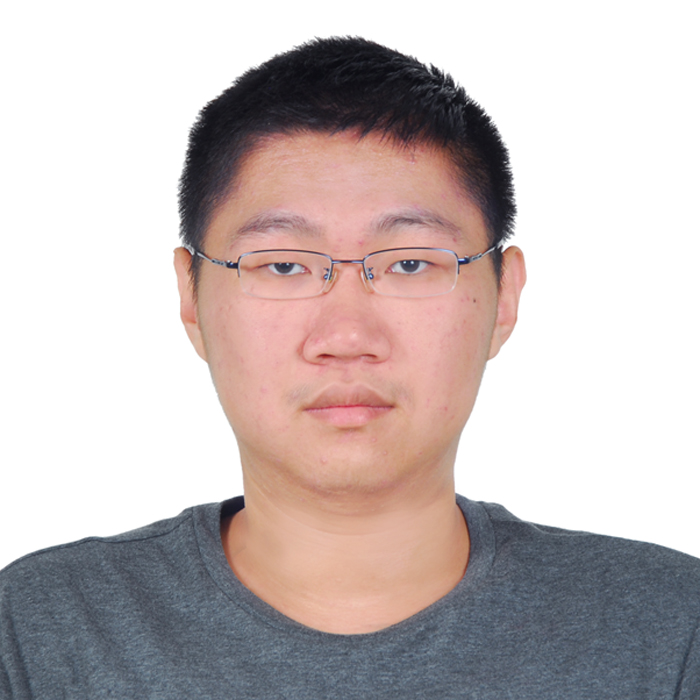
\includegraphics[width=1in,height=1.25in,clip,keepaspectratio]{./photo/xkz.jpg}}]{Kunze Xin} received his B.S. degree in Computer Science and Technology from Beijing University of Posts and Telecommunications, Beijing, China, in 2016. 
	He is currently pursuing the M.S. degree in Information Security at the Information Networking Institute, Carnegie Mellon University, Pittsburgh.
	His research interests include the computer-aided design for biochips and network security.
\end{IEEEbiography}

\vspace{-0.90cm}
\begin{IEEEbiography}[{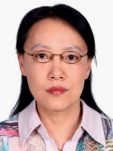
\includegraphics[width=1in,height=1.25in,clip,keepaspectratio]{./photo/caiyc.jpg}}]{Yici Cai} received B.S degree in Electronic Engineering from Tsinghua University, Beijing, China in 1983, received M.S. degree in Computer Science and Technology from Tsinghua University, Beijing, China in 1986, and received Ph.D in Computer Science, University of Science \& Technology of China, Hefei, China, in 2007. She has been a professor with the Department of Computer Science \& Technology, Tsinghua University. Her research interests include design automation for VLSI integrated circuits algorithms and theory, power/ground distribution network analysis and optimization, high performance clock synthesis, low power physical design.
\end{IEEEbiography}


\end{document}
